% - PER STILARE QUESTO DOCUMENTO VANNO INSERITI I DATI.
% - VISTO CHE IL FILE È LUNGO ED INTRICATO PER SEMPLIFICARE HO MESSO DEI COMMENTI
% - CHE INDICANO I PUNTI DOVE INSERIRE LE INFORMAZIONI CHE MANCANO.
% - INSERISCILI IN CORRISPONDENZA DEI COMMENTI:

% - "INSERT TITOLO"
% - "INSERT USO"
% - "INSERT DATA"
% - "INSERT DESCRIZIONE"
% - "INSERT INFORMAZIONI INCONTRO"
% - "INSERT DOMANDE E RISPOSTE" (intanto lo strutturiamo così, con domande e rispose, se servono altri tipi di struttura cambieremo)

% - "INSERT TITOLO" (verosimilmente sarà una cosa tipo "Verbale Esterno/Interno del xx/yy")
\usepackage{fix-cm}    

\makeatletter
\newcommand\HUGE{\@setfontsize\Huge{40}{50}}
\makeatother    
 
\newcommand{\Titolo}{Neuradillo}

\newcommand{\Gruppo}{Giovanni Sorice \\
Francesco Corti}

\newcommand{\Versione}{1.0.0}

\newcommand{\Redazione}{}




\documentclass[a4paper, oneside, openany]{article}

\usepackage{graphbox}
% permette di modificare i margini
\usepackage[top=3.1cm, bottom=3.1cm, left=2.2cm, right=2.2cm]{geometry}

\usepackage{lastpage} %info sul # dell'ultima pagina del documento
\usepackage{fancyhdr} %per modificare dimensioni,margini, intestazioni e righe a piè di pagina
\fancypagestyle{plain}{
  % cancella tutti i campi di intestazione e piè di pagina
  \fancyhf{}
  
  %\lfoot{ %piè di pagina
   %{\Titolo} \ - \textit{{\Gruppo}}
  %}
  \rfoot{Pagina \thepage{} di \pageref{LastPage}} %es: pag: 4 di 10

  %linea orizzontale alle posizioni top e bottom della pagina
  \renewcommand{\headrulewidth}{0.2	pt}  
  \renewcommand{\footrulewidth}{0.2pt}
}
\pagestyle{plain}

%Comando Spazio
\newcommand{\Spazio}{\mbox{} \\ \mbox{} \\ }  


%\usepackage{calc} %introduce la notazione infissa per le op. aritmetiche interne a LaTeX

\usepackage[utf8]{inputenc}
\usepackage[T1]{fontenc}
\usepackage[italian]{babel} %il documento è in italiano
%\usepackage{textcomp} %The pack­age sup­ports the Text Com­pan­ion fonts, which pro­vide many text sym­bols
%(such as baht, bul­let, copy­right, mu­si­cal­note, onequar­ter, sec­tion, and yen), in the TS1 en­cod­ing.

\usepackage{graphicx}       %permette di inserire delle immagini
\usepackage{caption}        %numerazione figure e loro descrizione testuale
\usepackage{subcaption}     %sottofigure numerabili
\usepackage{float}  %permette di inserire un # qualsiasi di figure fluttuanti
\usepackage{xcolor}
\usepackage{rotating} %permette di ruotare le immagini
%\usepackage{changepage} %utile se c'è bisogno di aggiustare margini per centrare figure

%package utili per la math mode ( $ ... $ o \[ ...  )
\usepackage{amsmath}
\usepackage{amssymb}
\usepackage{amsfonts}
%\usepackage{euler}    %font 'ams euler', lo stesso di 'Concrete Mathematics' di Knuth
\usepackage{amsthm}
\usepackage{mathtools}

% package utili per tabelle(\thead in particolare)
\usepackage{array, booktabs, caption}
\usepackage{makecell}
\renewcommand\theadfont{\bfseries}
\usepackage{boldline}

\usepackage{listings} %permette di inserire degli spezzoni di codice

\usepackage{tikz} %disegno di immagini vettoriali a schermo. Utile per grafi
\usetikzlibrary{arrows.meta}
\usetikzlibrary{graphs}
\usetikzlibrary{arrows}
%\usepackage{tikz-uml} %serve per disgnare l'UML, fantastica guida:
%https://perso.ensta-paristech.fr/~kielbasi/tikzuml/var/files/doc/tikzumlmanual.pdf
%download package: http://perso.ensta-paristech.fr/~kielbasi/tikzuml/

%package per le tabelle
\usepackage{booktabs} %permette di poter usare delle liste nelle tabelle
\usepackage{tabularx} 
\usepackage{longtable} %una tabella può continuare su più pagine
\usepackage{multirow} %utile per visualizzare una cella su più righe
%\usepackage{multicolumn} %cella su più colonne
%\usepackage[table]{xcolor} %rende disponibile l'utilizzo di un colore per lo sfondo
                        %delle celle di una tabella

%crea una cella per le tabelle in grado di andare a capo con \newline
%https://tex.stackexchange.com/questions/12703/how-to-create-fixed-width-table-columns-with-text-raggedright-centered-raggedlef
\usepackage{array}
\newcolumntype{L}[1]{>{\raggedright\let\newline\\\arraybackslash\hspace{0pt}}m{#1}}
\newcolumntype{C}[1]{>{\centering\let\newline\\\arraybackslash\hspace{0pt}}m{#1}}
\newcolumntype{R}[1]{>{\raggedleft\let\newline\\\arraybackslash\hspace{0pt}}m{#1}}


%indice con i puntini
\usepackage{tocloft}
\renewcommand\cftsecleader{\cftdotfill{\cftdotsep}}

%http://ctan.mirror.garr.it/mirrors/CTAN/macros/latex/contrib/appendix/appendix.pdf
\usepackage{appendix} %aggiunge dei comandi per l'appendice
\usepackage{parskip} %aiuta LaTeX a trovare il miglior stile per i page break
\setcounter{secnumdepth}{5} % numera i sottoparagrafi
\setcounter{tocdepth}{5} %aggiunge all'indice i sottoparagrafi
%\usepackage{titlesec} %\begin{paragraph} si può usare come subsubsubsection!


\usepackage{breakurl}%\url{...} può continare alla linea successiva. (si può andare a capo)

\definecolor{Maroon}{cmyk}{0, 0.87, 0.68, 0.32}
\usepackage[colorlinks=true]{hyperref}
\hypersetup{
    colorlinks=true,
    citecolor=black,
    filecolor=black,
    linkcolor=black, % colore dei link interni
    urlcolor=Maroon  % colore dei link interniesterni
}

%impostazioni per il codice che deve finire dentro a
%\begin{lstlisting}

\definecolor{listinggray}{gray}{0.9}
\definecolor{lbcolor}{rgb}{0.9,0.9,0.9}
\lstset{
backgroundcolor=\color{lbcolor},
    tabsize=4,    
%   rulecolor=,
    language=[GNU]C++,
    basicstyle=\scriptsize,
    upquote=true,
    aboveskip={1.5\baselineskip},
    columns=fixed,
    showstringspaces=false,
    extendedchars=true,
    inputencoding=utf8,
    breaklines=true,
    prebreak = \raisebox{0ex}[0ex][0ex]{\ensuremath{\hookleftarrow}},
    frame=single,
    numbers=left,
    showtabs=false,
    showspaces=false,
    showstringspaces=false,
    identifierstyle=\ttfamily,
    keywordstyle=\color[rgb]{0,0,1},
    commentstyle=\color[rgb]{0.026,0.112,0.095},
    stringstyle=\color[rgb]{0.627,0.126,0.941},
    numberstyle=\color[rgb]{0.205, 0.142, 0.73},
%        \lstdefinestyle{C++}{language=C++,style=numbers}’.
}
\lstset{
  backgroundcolor=\color{lbcolor},
  tabsize=4,
  language=C++,
  captionpos=b,
  tabsize=3,
  frame=lines,
  numbers=left,
  numberstyle=\tiny,
  numbersep=5pt,
  breaklines=true,
  showstringspaces=false,
  basicstyle=\footnotesize,
  identifierstyle=\color{magenta},
  keywordstyle=\color[rgb]{0,0,1},
  commentstyle=\color{orange},
  stringstyle=\color{red}
}


 \newgeometry{top=4cm}

\begin{document}

\begin{titlepage}
	\begin{center}
		
		\begin{center}
			%% qui metteteci l'immagine di copertina. Io ho messo quella dell'uni,
			%voi mettete quella del vostro grupo
			%\includegraphics[scale=0.8]{RO/fig/logo_unipi.png}
		\end{center}
		
		\vspace{1cm}
	
		\begin{HUGE}
		
			\textbf{\Titolo{}} \\
		\end{HUGE}
		
		\vspace{13pt}  
		
		\begin{large}
		\Gruppo{}\ \\	
		\end{large}
		
		\vspace{5pt}  
		
		\begin{large}
		f.corti3@studenti.unipi.it \\
		g.sorice@studenti.unipi.it \\
		\end{large}
		
		\vspace{5pt}  
		
		\begin{large}
			Machine Learning A.A. 2019-2020 \\
		\end{large}	
		
		\vspace{5pt}
		    
		\begin{large}
			Date: \textit{28/01/2020}		 \\
		\end{large}
		
		\vspace{5pt}
		  		
		\begin{large}
			Type of project: \textbf{A} 
		\end{large}	  
		
	\end{center}
\end{titlepage}

\restoregeometry


\section{Abstract}
The aim of the following document is to illustrate the work done for the assignment. Firstly exposing the development choices and showing then the result of the tests.
\section{Experiments}


\subsection{MONK's results}

The neural network used for the problems have 17 input units, the number of hidden units as written in the table \ref{tab:dati} and 1 output units. We used \texttt{tanh} as hidden layer activation function and \texttt{sigmoid} as output layer activation function. We chose \texttt{Mean squared error} as loss function. An input is classified as 1 if the output of the neural network is greater than 0.5 or 0 otherwise.\\
We used stochastic, mini-batch and batch gradient descent but in the end we decided to use the batch gradient descent because loss function plots were smoother than the others.
We also used the weight decay regularization as lambda parameter and Nesterov momentum as momentum parameter. The table \ref{tab:dati} reports the average of the value found for TR and TS after five different trainings of the networks.    
\begin{center}
\small\addtolength{\tabcolsep}{-5pt}
\begin{table}[H]
\begin{tabular}{|c|c|c|c|c|c|c|}
\hline
\textbf{Task} &	\textbf{\#Units} &\textbf{ eta} & \textbf{lambda} &\textbf{momentum} & {\textbf{MSE(TR/TS)}} &\textbf{Accuracy(TR/TS)} \\ \hline
MONK 1        &    3 & 0.9 & 0 & 0.7  &   6.3e-4/1e-3 &   100\%/100\%  \\ \hline
MONK 2        &    4 & 0.8 & 0 & 0.7  &   1e-3/1.3e-3 &   100\%/100\% \\ \hline               
MONK 3        &    5 & 0.4 &5e-3 &0.2&     7.8e-2/5.5e-2&    93.44\%/97.22\%  \\ \hline
MONK 3 (no reg)&   5 & 0.6 &   0 &  0.7 &   1.7e-2/2.7e-2 & 95.90\%/93.51\%		\\ \hline              
\end{tabular}
\caption{MONK's problems parameter and results.}
\label{tab:dati}
\end{table}
\end{center}
\subsubsection{MONK 1}

\begin{figure}[H]
    \centering
    \begin{minipage}[t]{0.5\linewidth}
        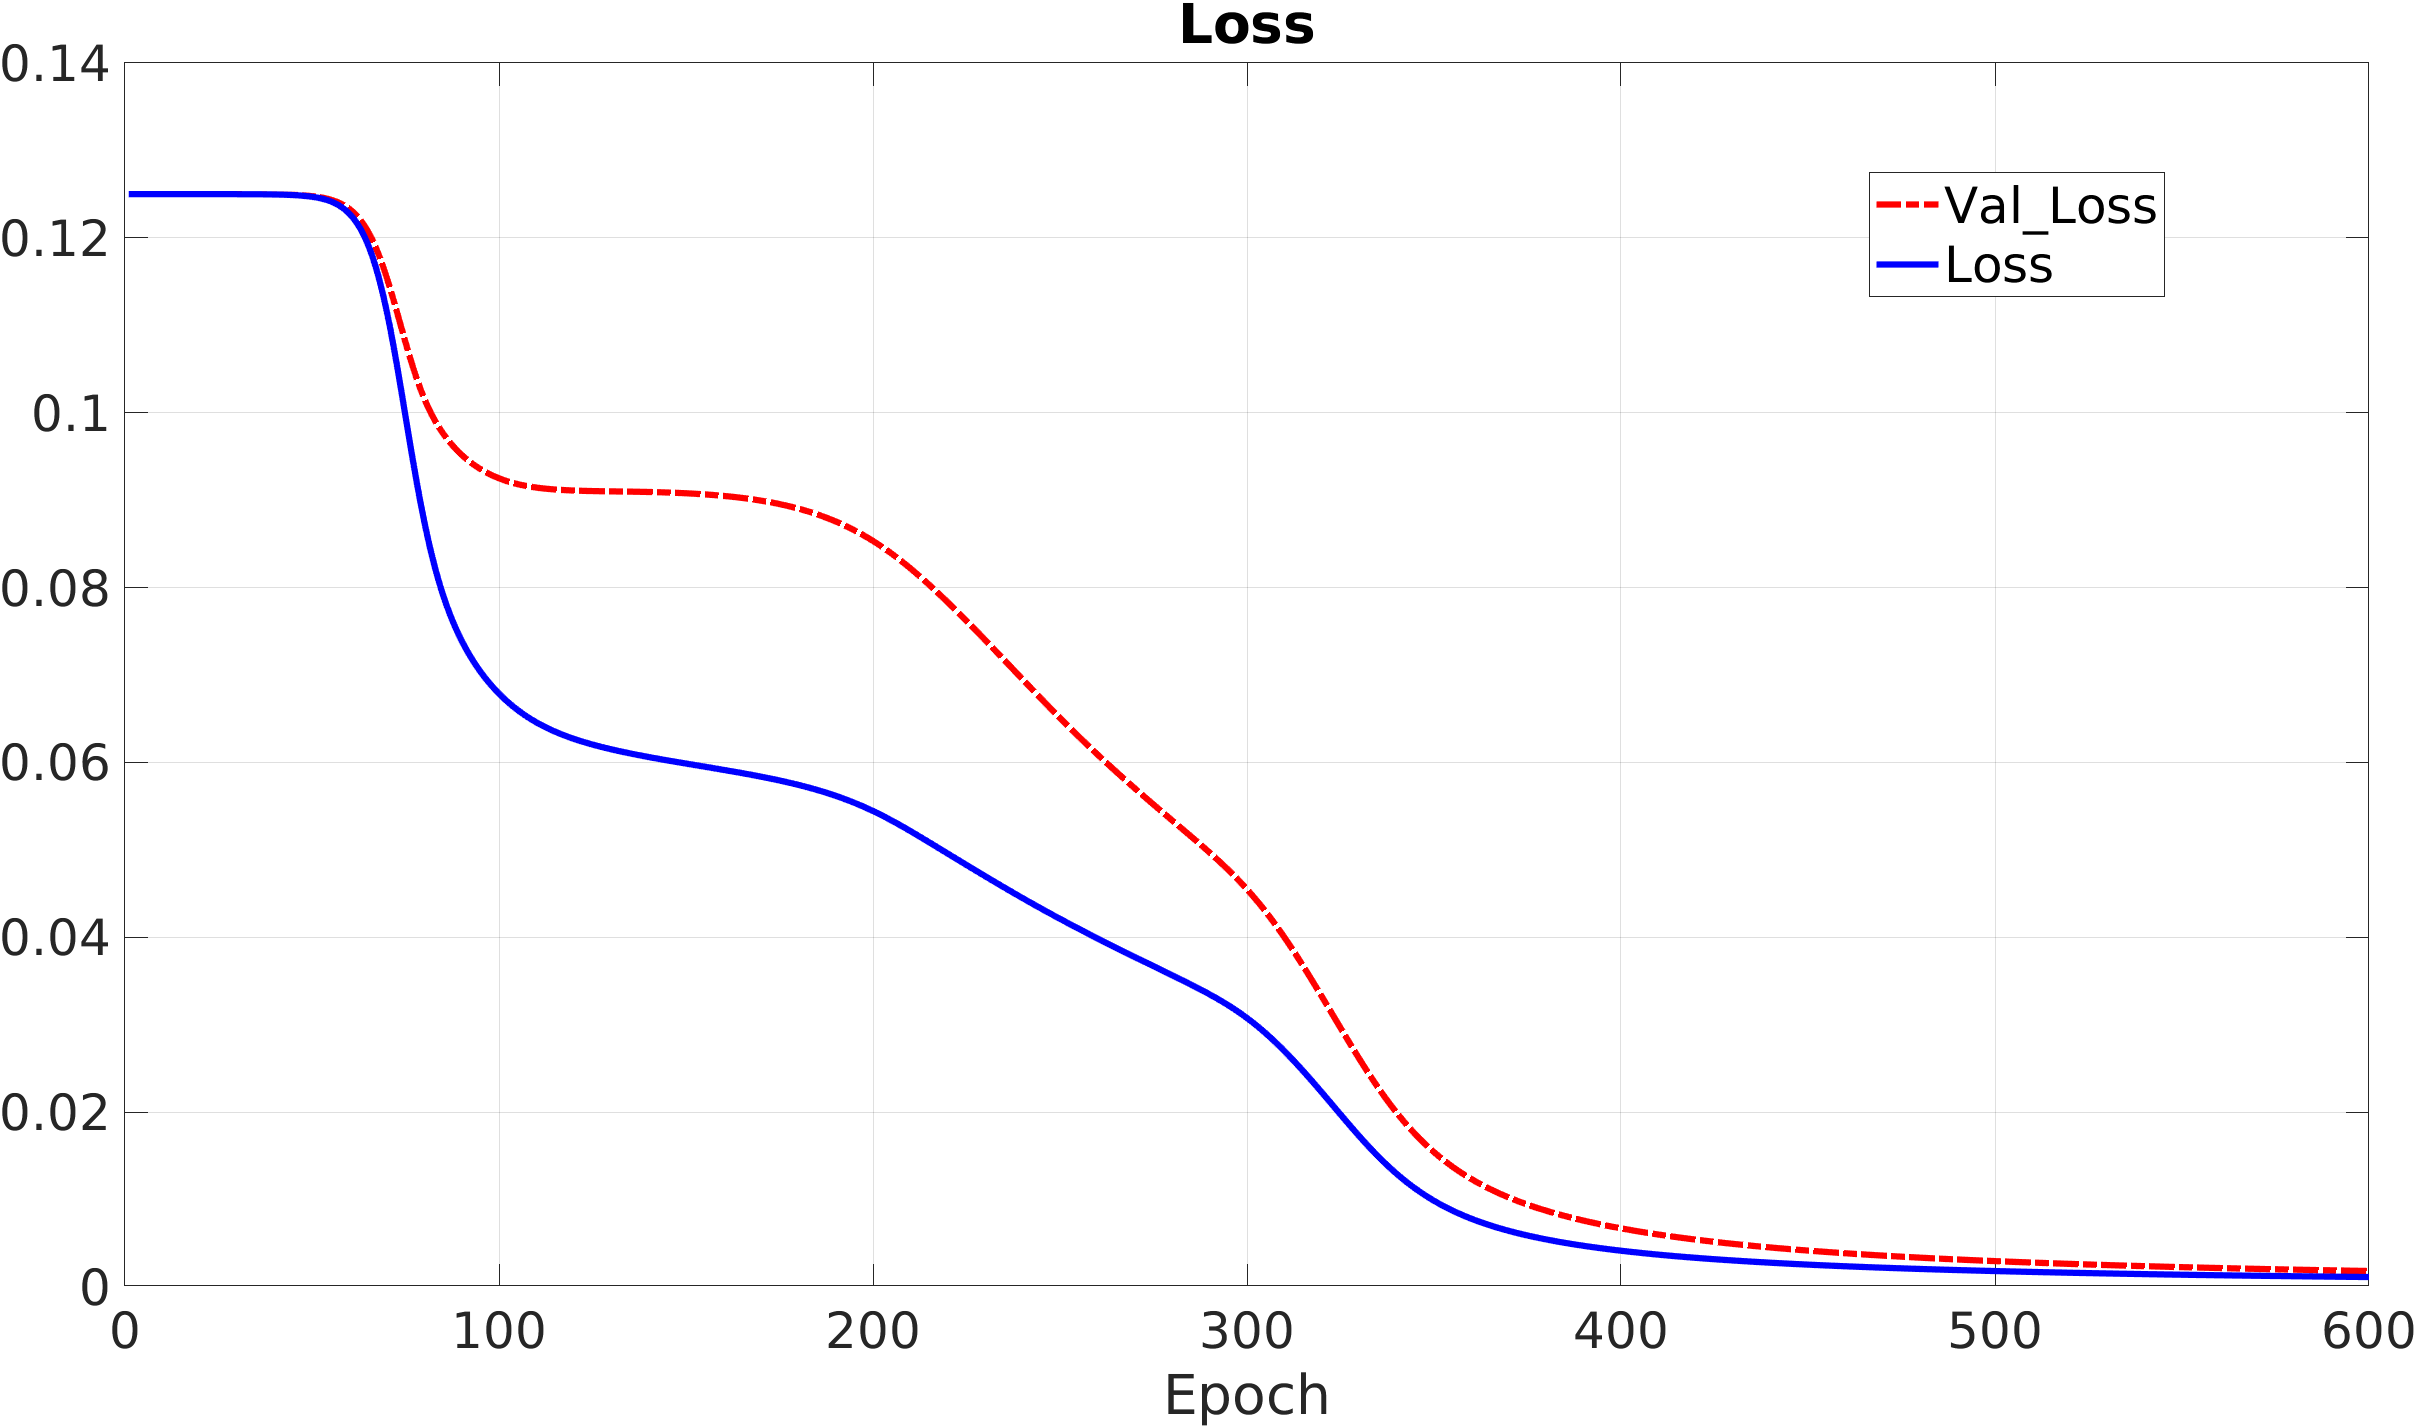
\includegraphics[width=\linewidth]{img/Monk1_loss.png}
        %\subcaption{MSE}
    \end{minipage}%
    \begin{minipage}[t]{0.5\linewidth}
        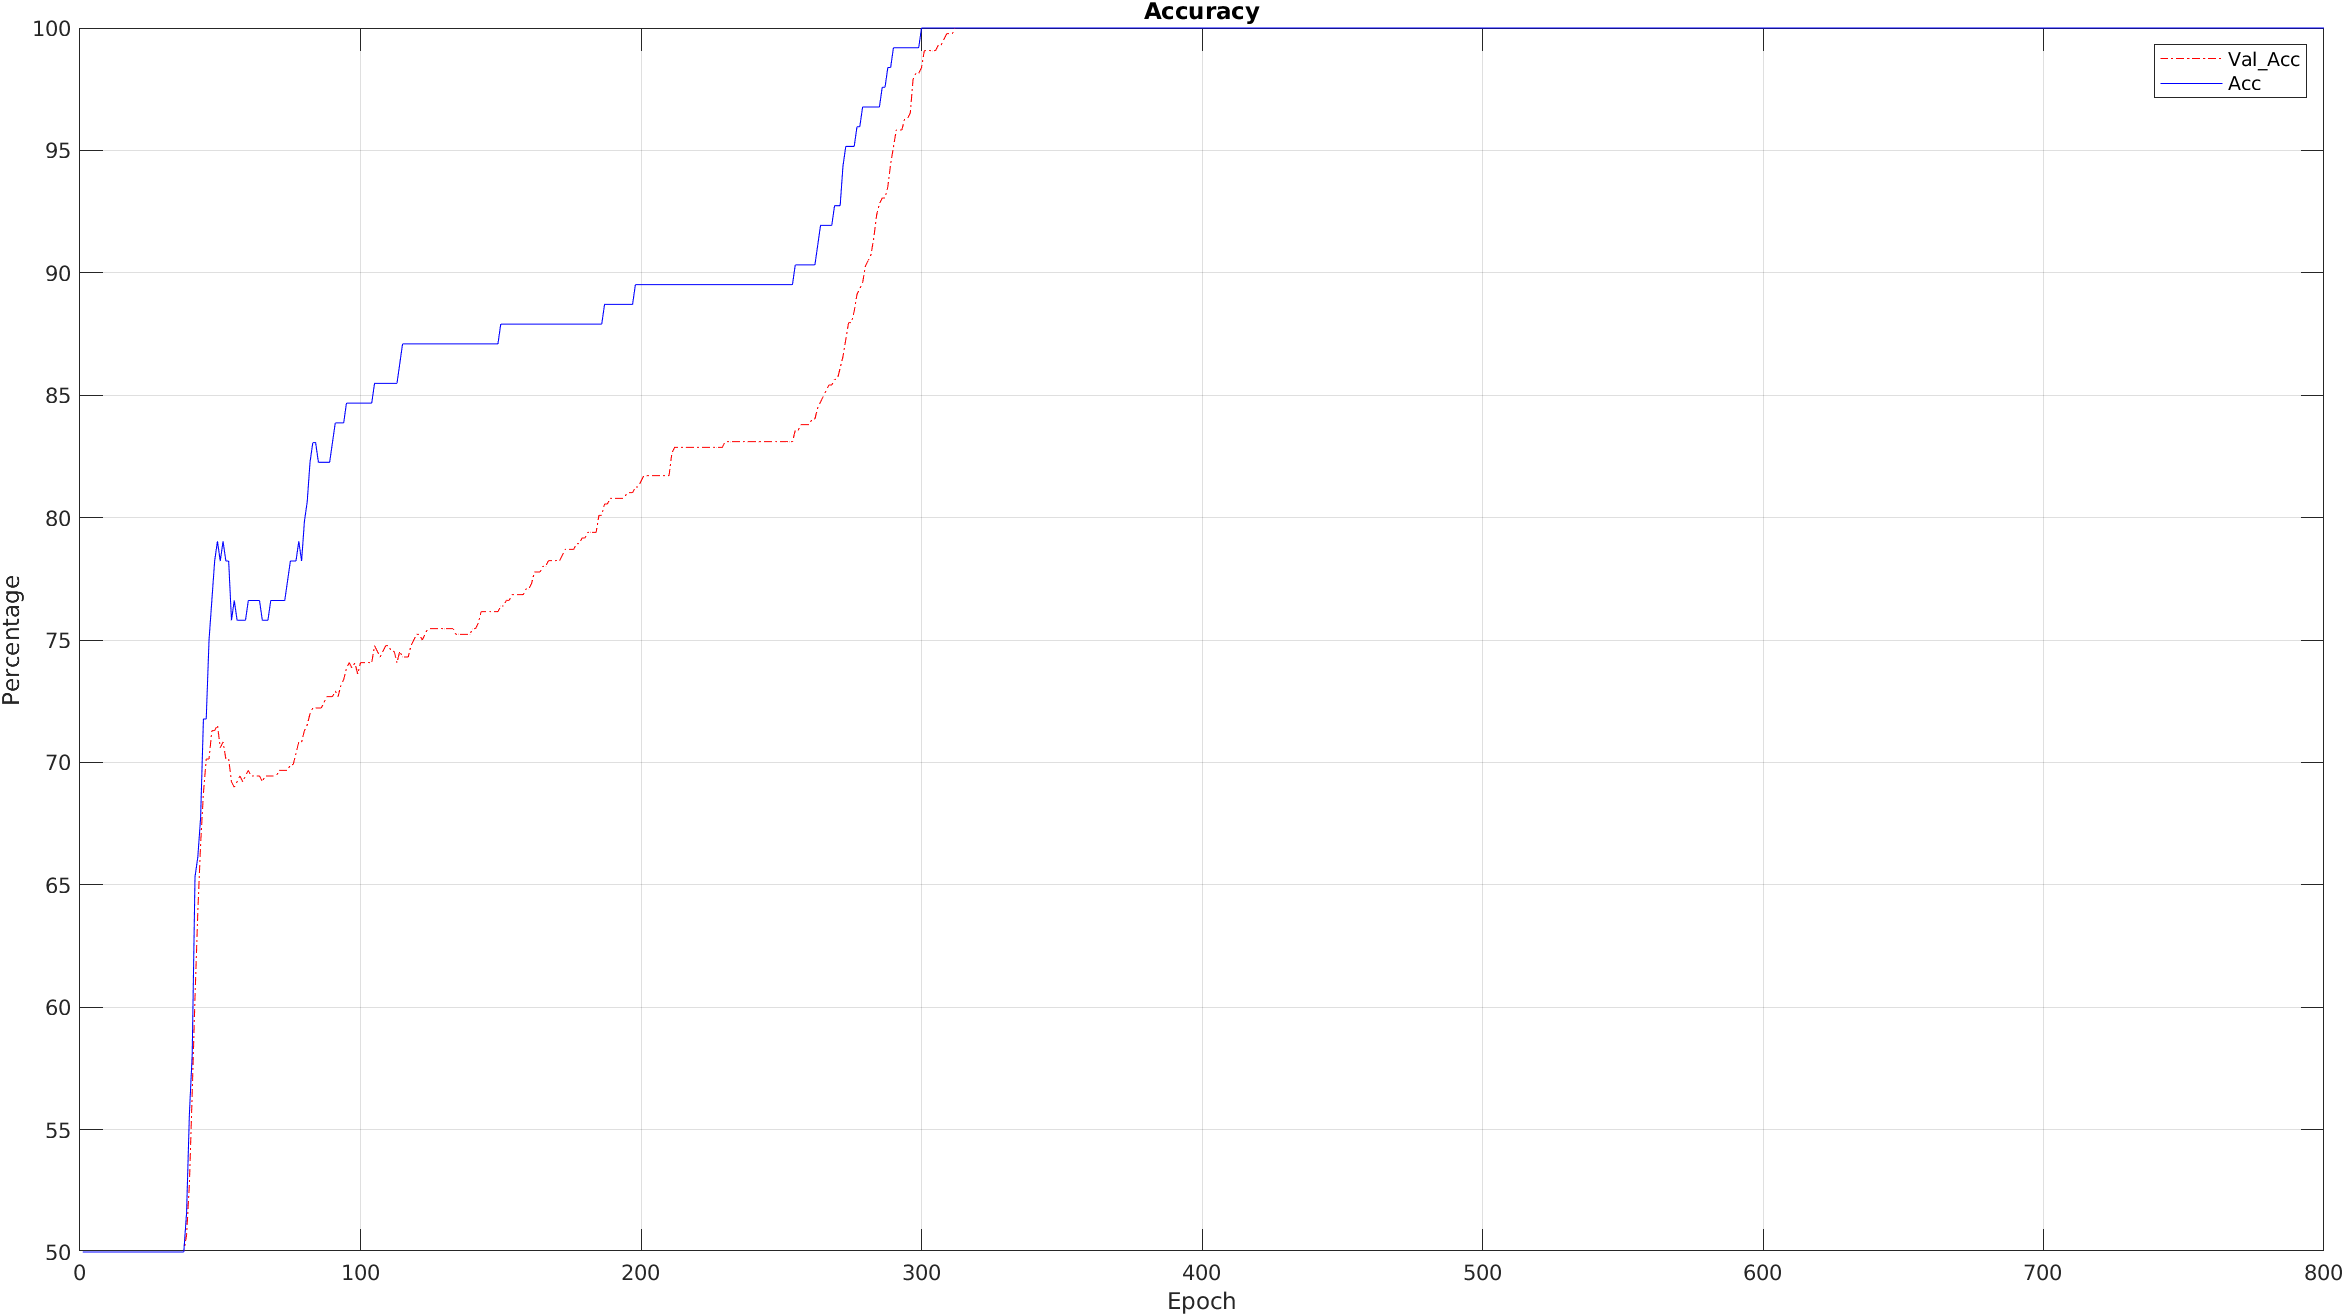
\includegraphics[width=\linewidth]{img/Monk1_accuracy.png}
        %\subcaption{Accuracy}
    \end{minipage}
    \caption{MSE and accuracy for MONK’s 1.}
\end{figure}

\subsubsection{MONK 2}
\begin{figure}[H]
    \centering
    \begin{minipage}[t]{0.5\linewidth}
        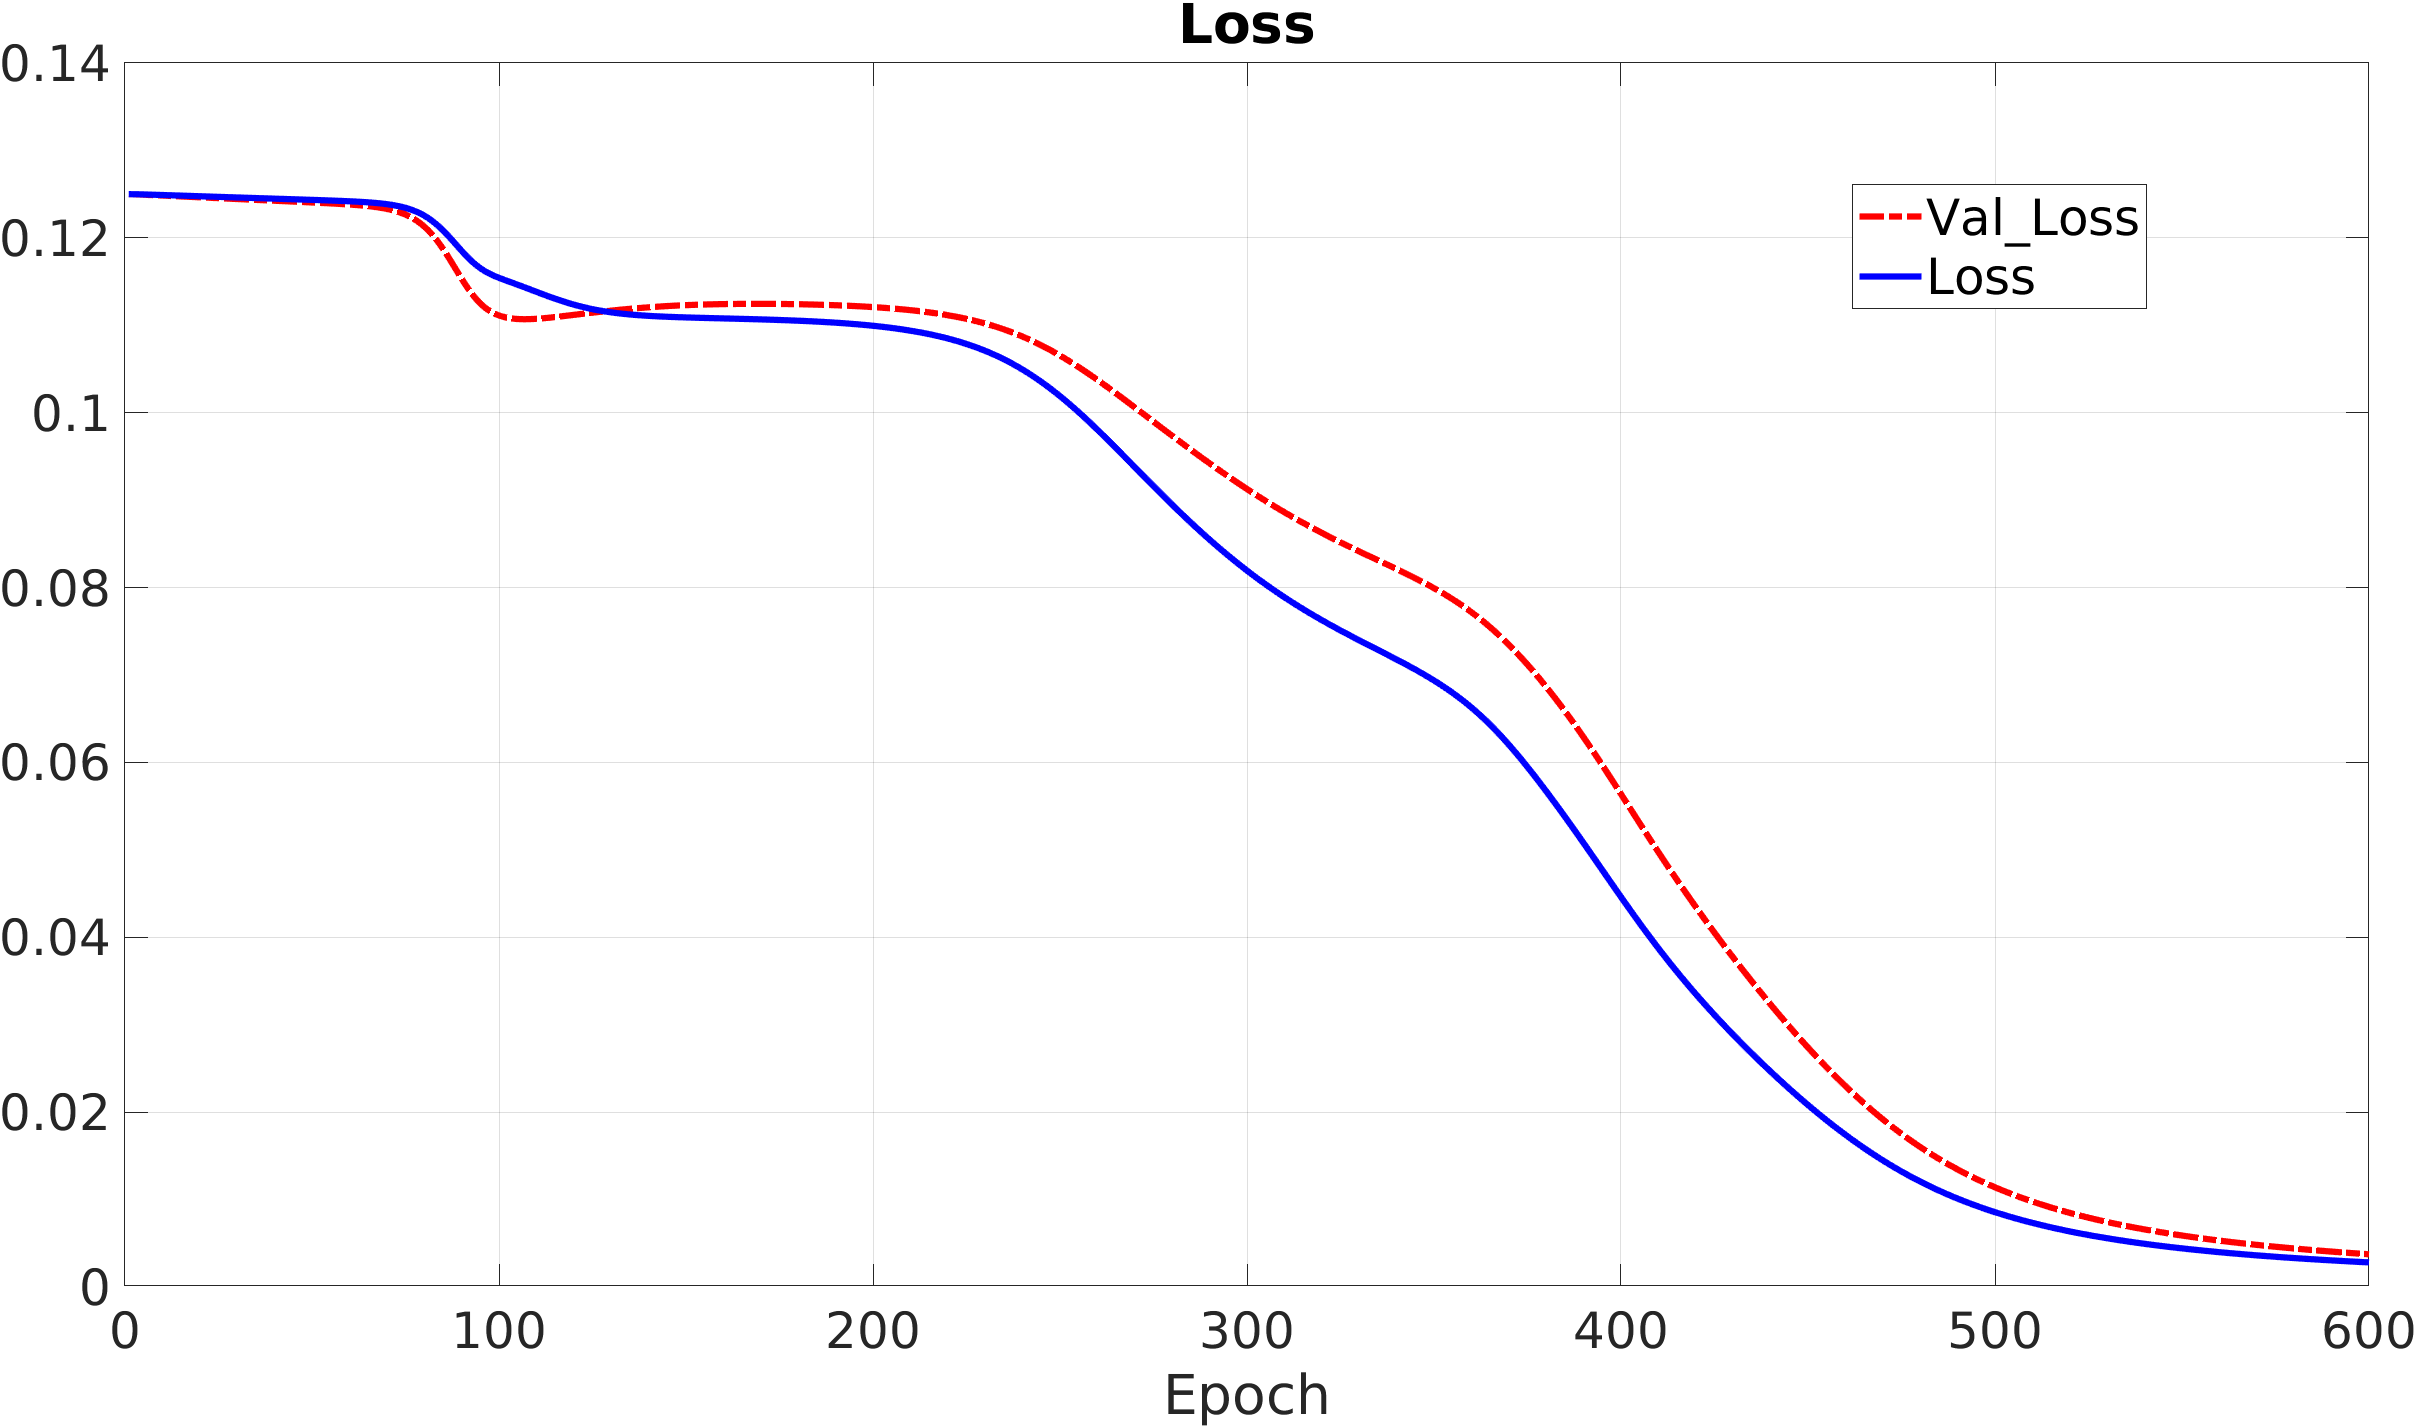
\includegraphics[width=\linewidth]{img/Monk2_loss.png}
        %\subcaption{MSE}
    \end{minipage}%
    \begin{minipage}[t]{0.5\linewidth}
        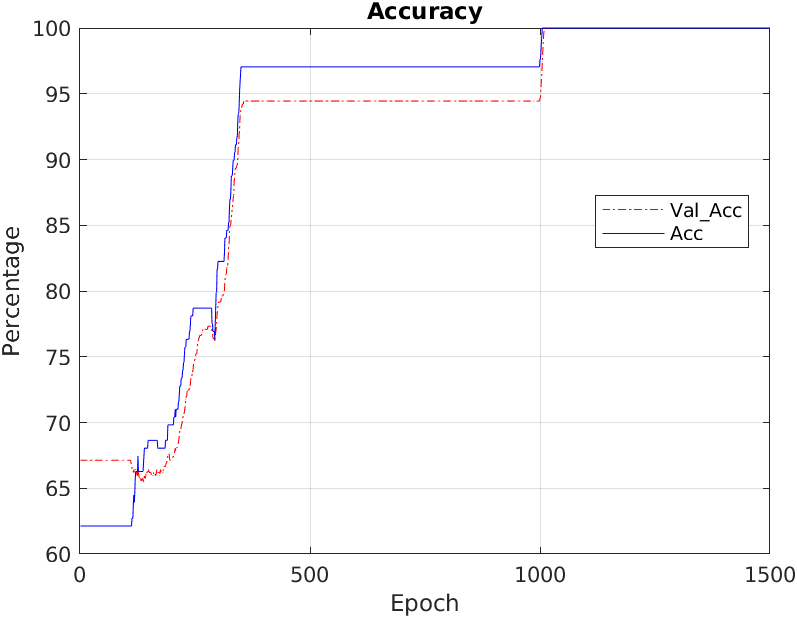
\includegraphics[width=\linewidth]{img/Monk2_accuracy.png}
        %\subcaption{Accuracy}
    \end{minipage}
    \caption{MSE and accuracy for MONK’s 2.}
\end{figure}

\subsubsection{MONK 3}
We figured out during training phase that learning curves of MONK's 3 without regularization shown overfits in the output (see fig. \ref{fig:m3nr}). After that we tried with regularization and we obtained better results, the training didn't show overfitting in the validation error.
\begin{figure}[H]
    \centering
    \begin{minipage}[t]{0.5\linewidth}
        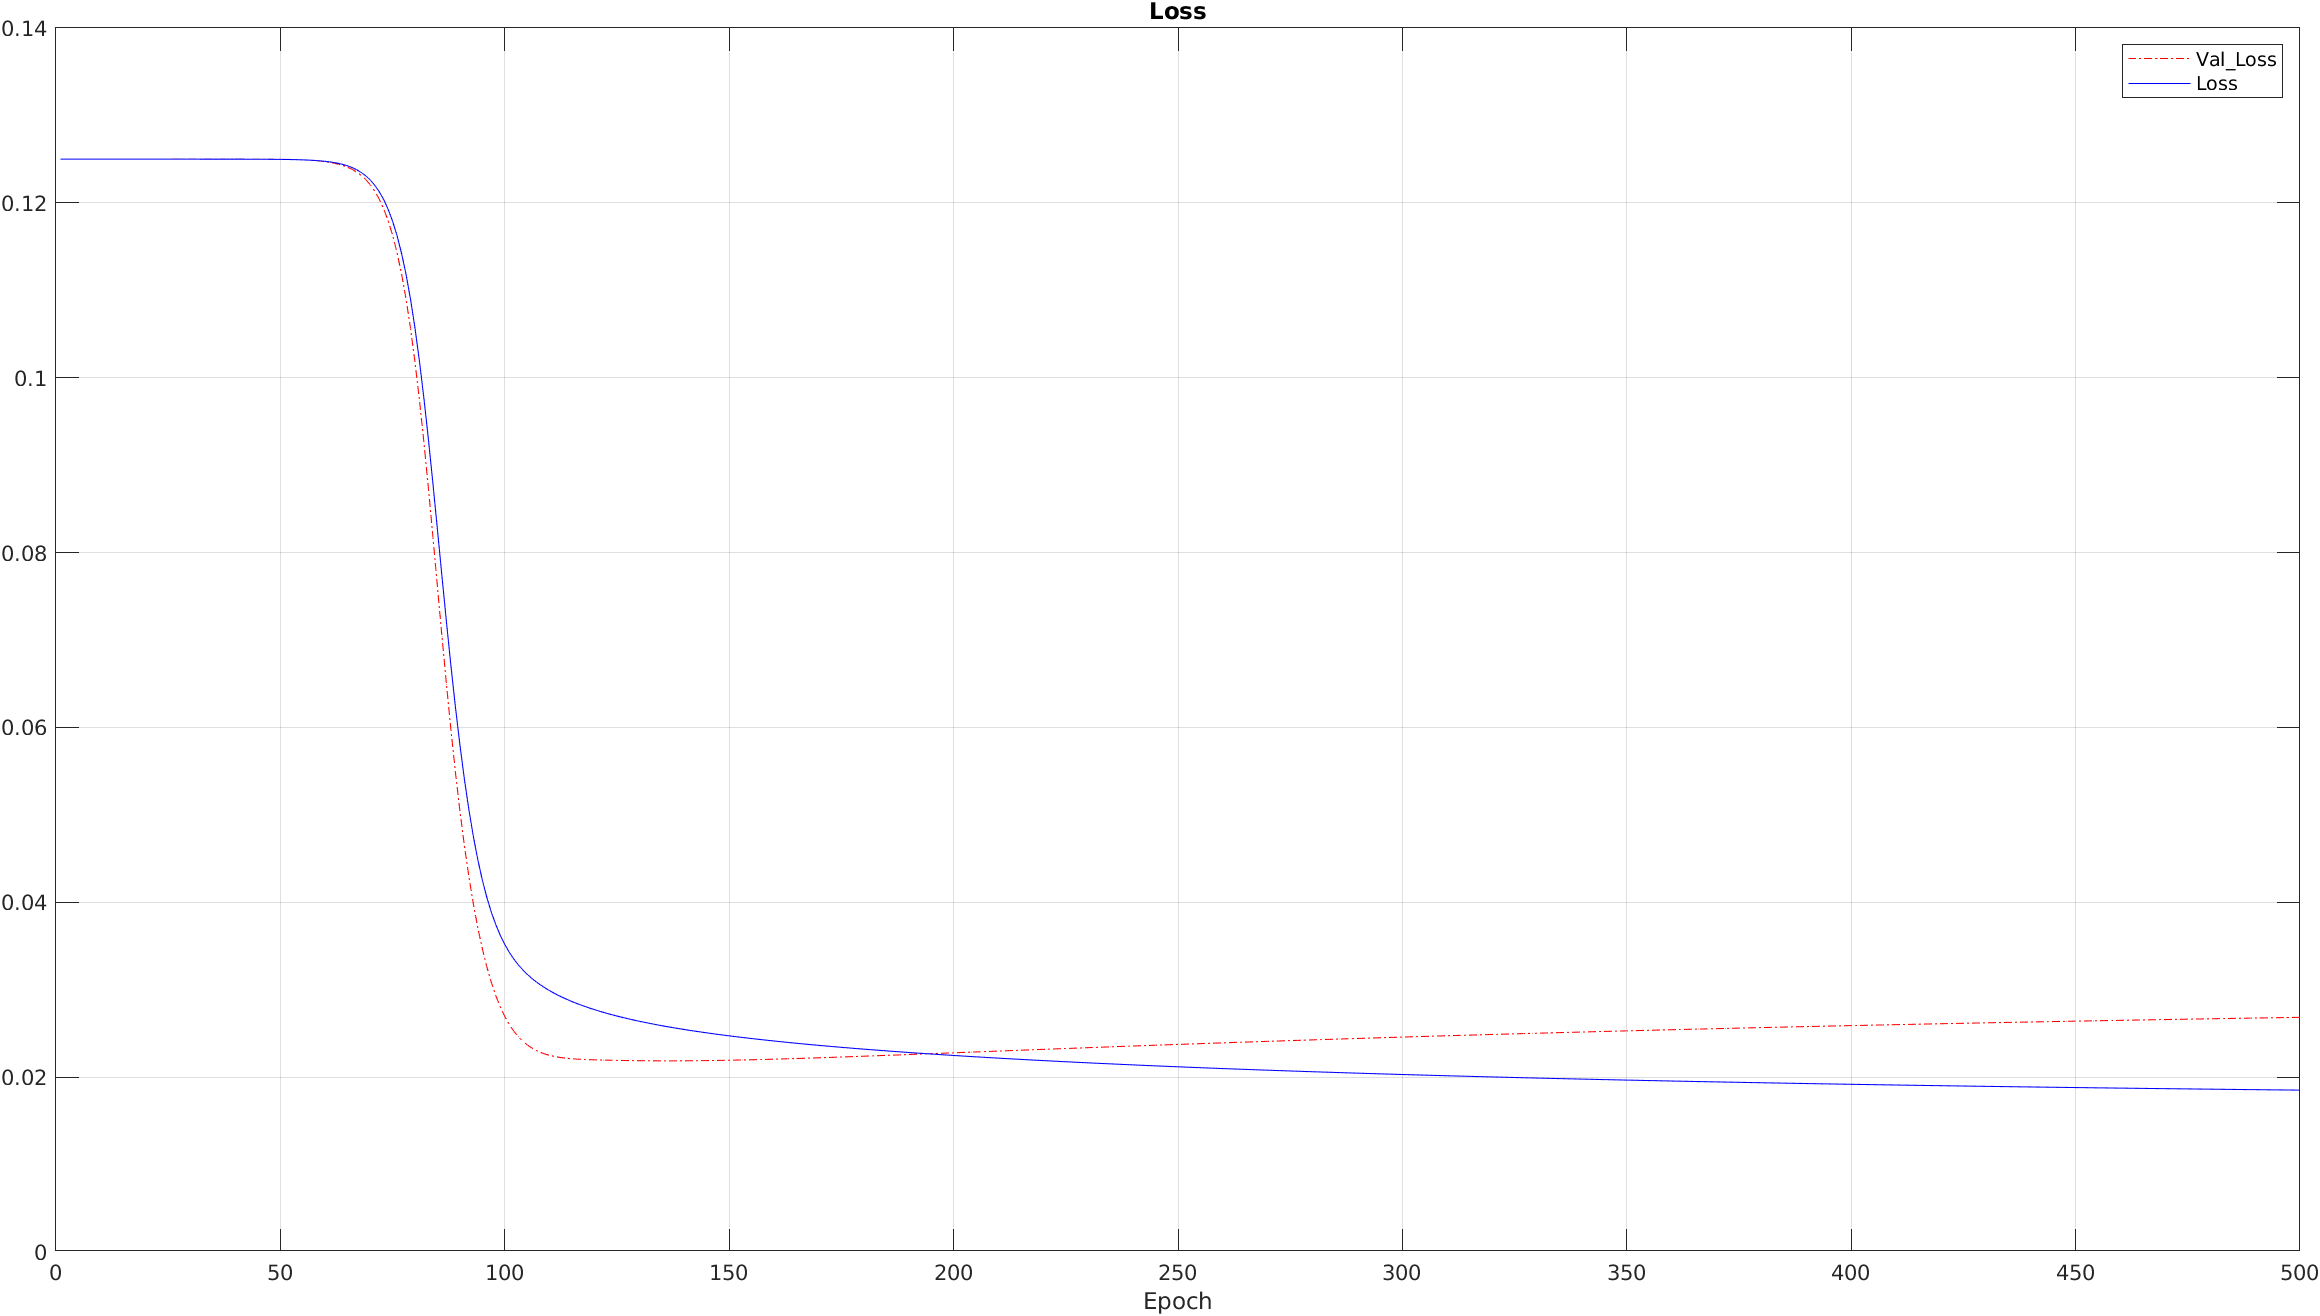
\includegraphics[width=\linewidth]{img/Monk3_loss_noReg.png}
        %\subcaption{MSE}

    \end{minipage}%
    \begin{minipage}[t]{0.5\linewidth}
        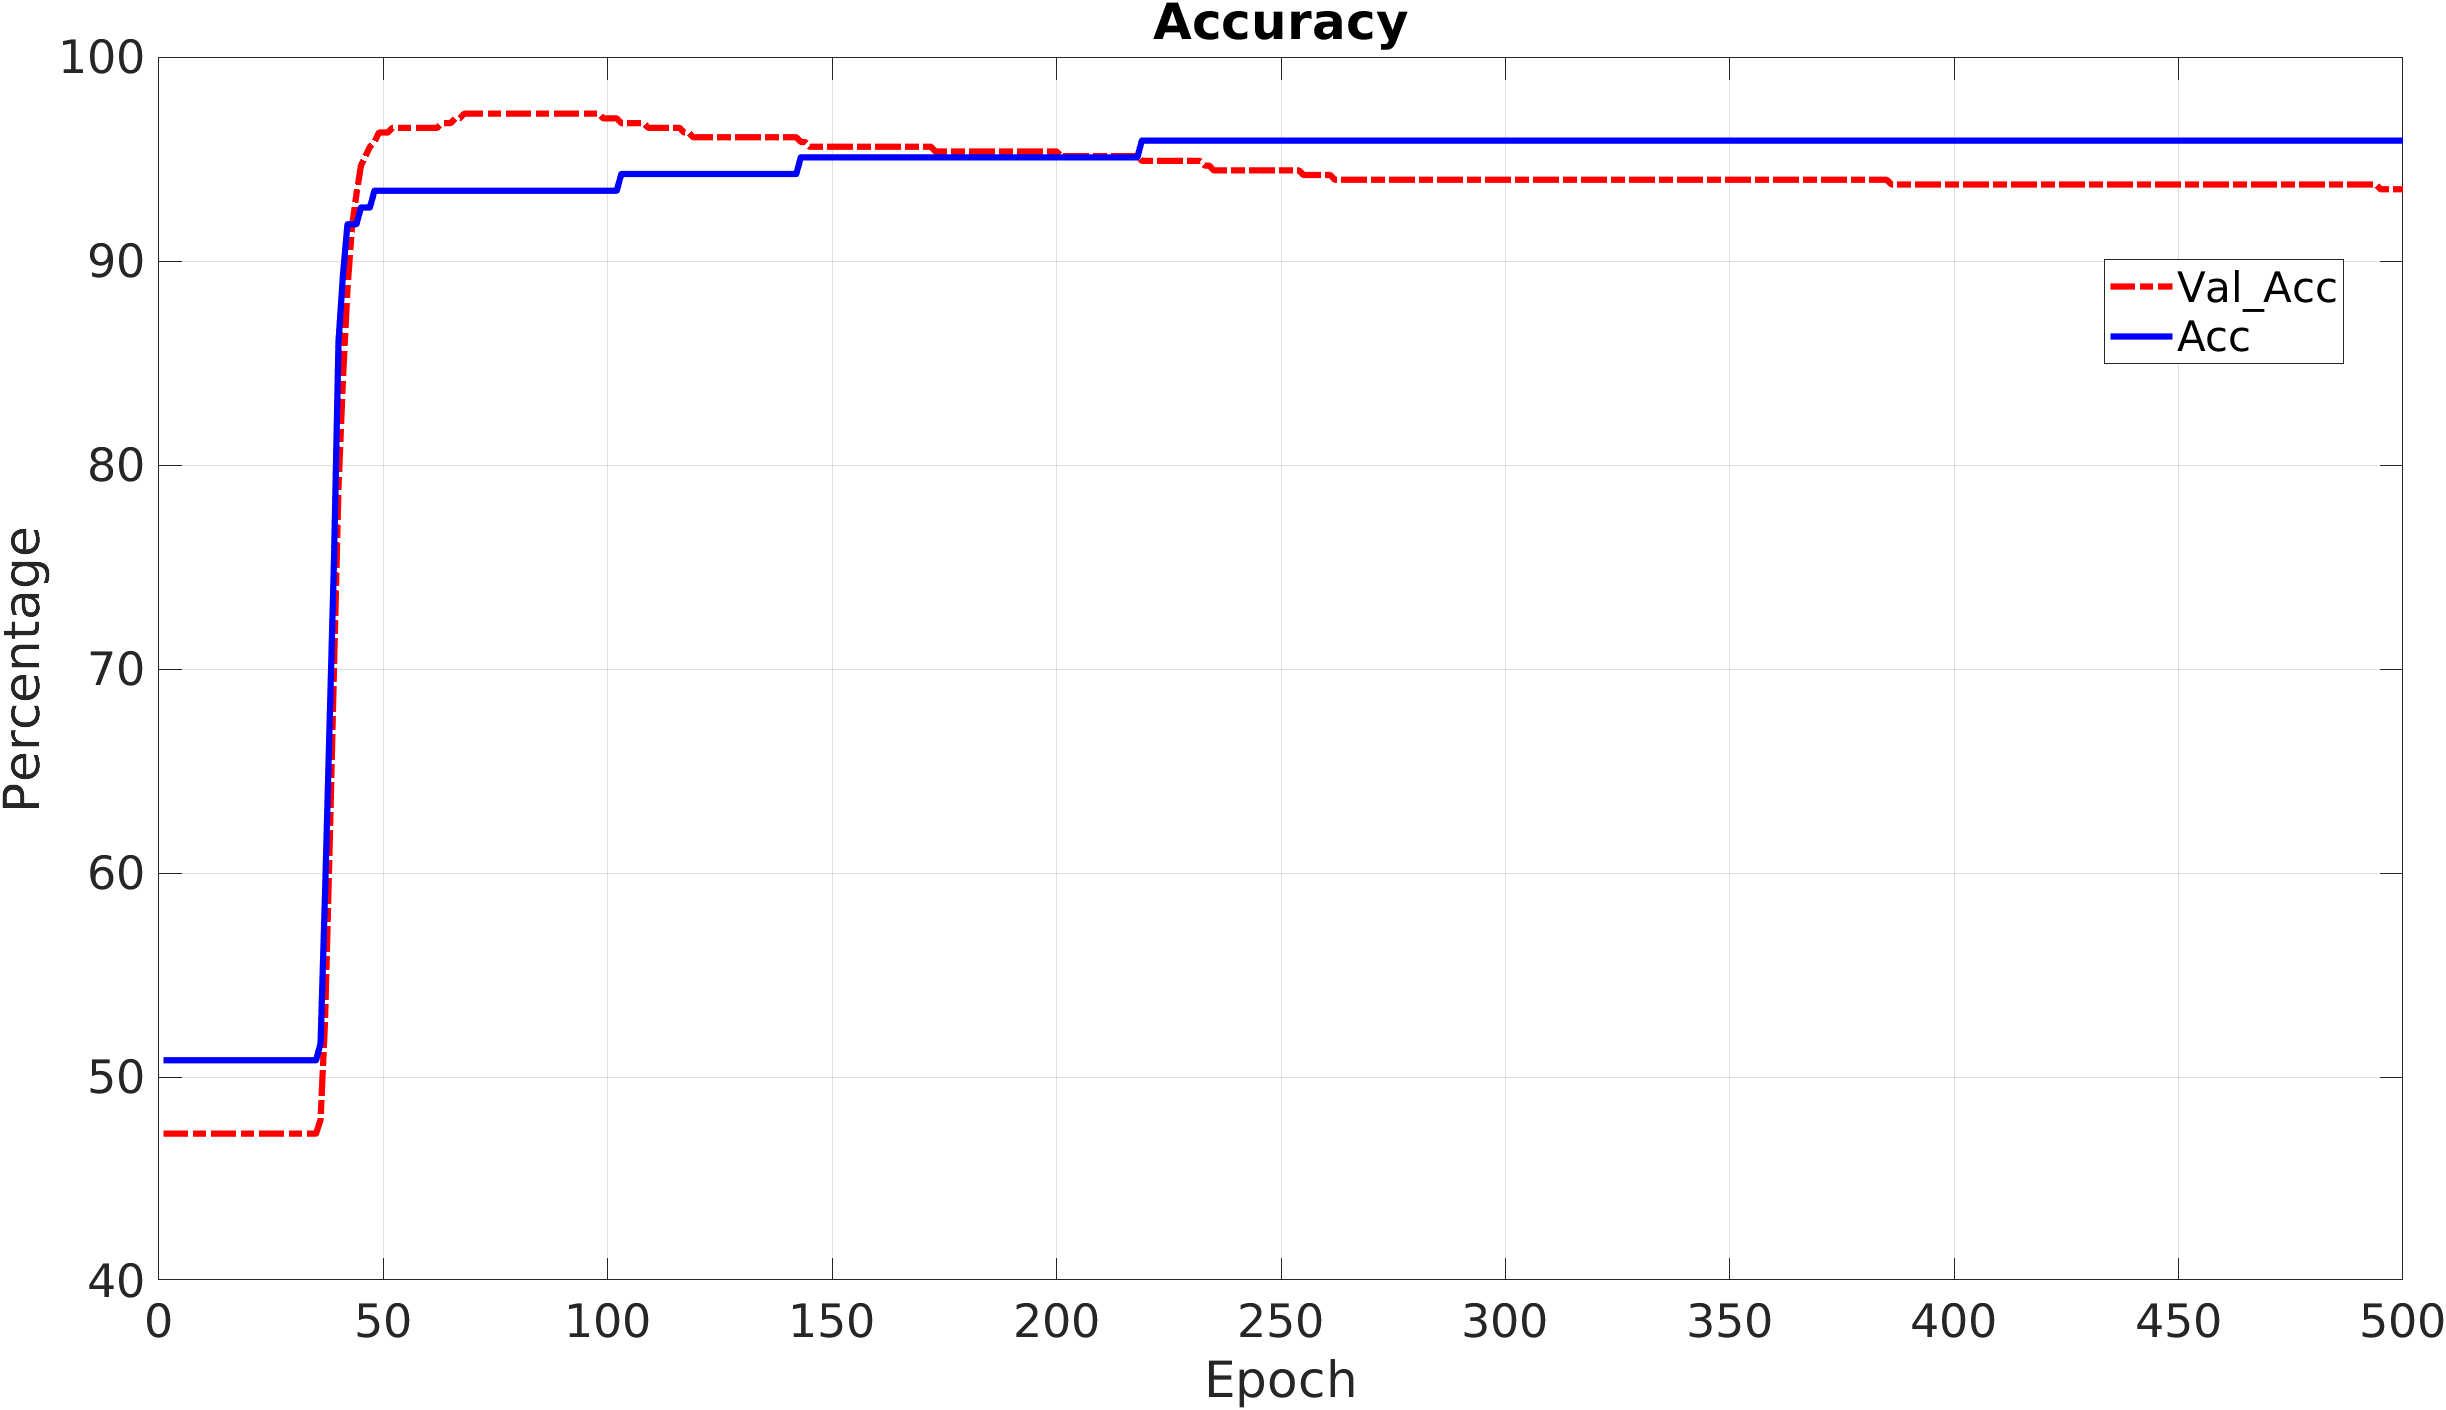
\includegraphics[width=\linewidth]{img/Monk3_accuracy_noReg.png}
        %\subcaption{Accuracy}
    \end{minipage}
    \caption{MSE and accuracy for MONK’s 3 not regularized.}
    \label{fig:m3nr}
\end{figure}

\begin{figure}[H]
    \centering
    \begin{minipage}[t]{0.5\linewidth}
        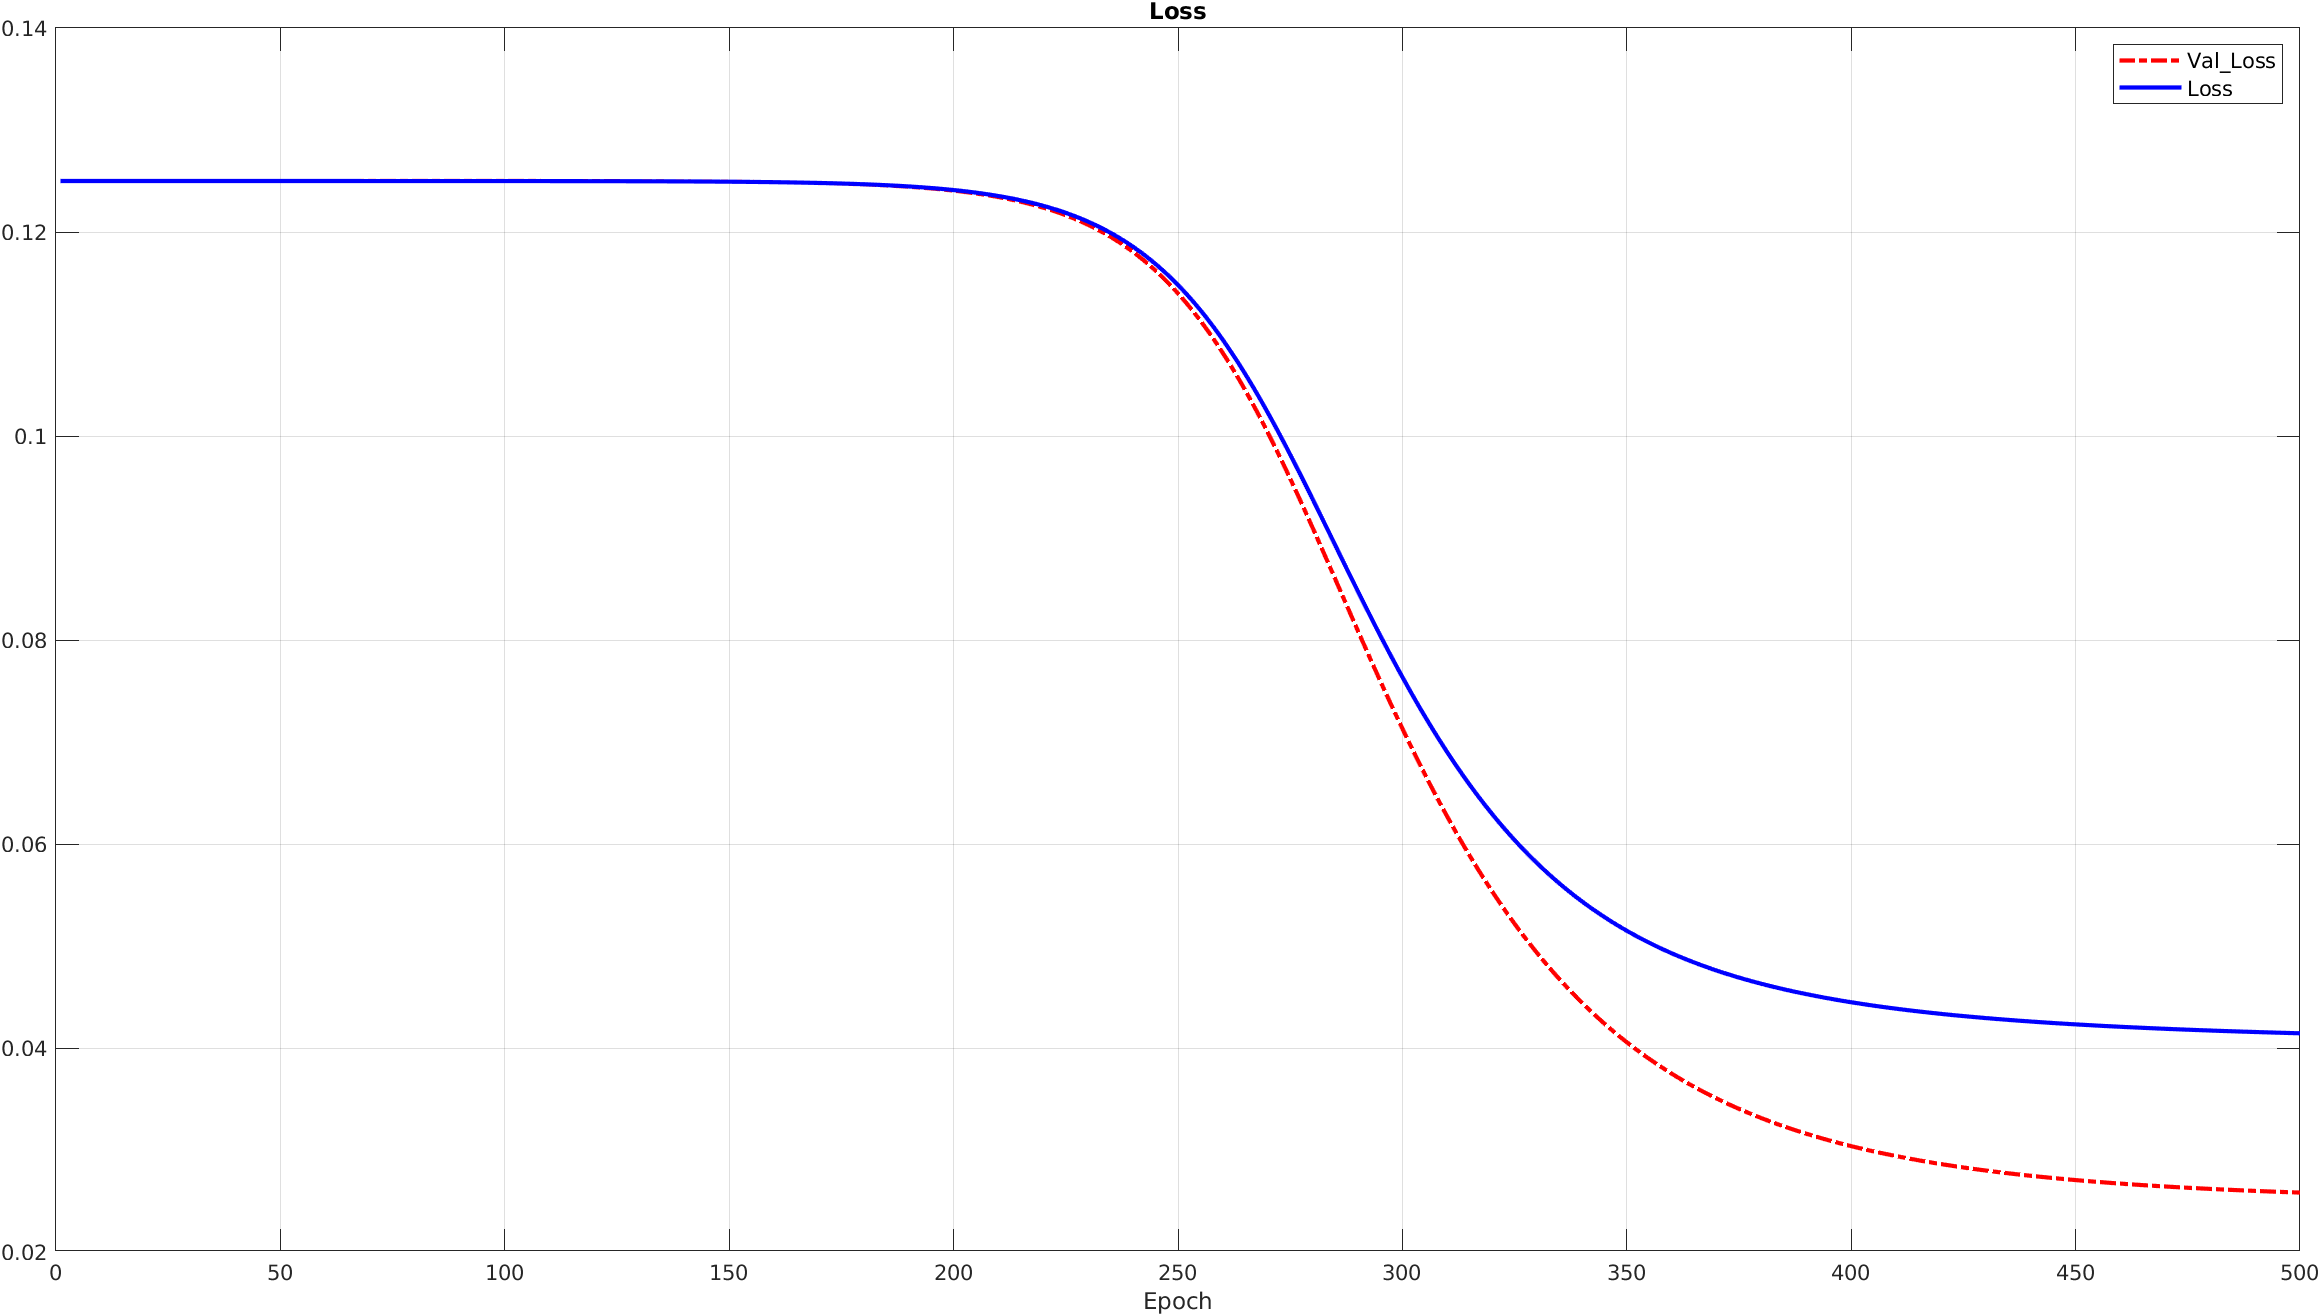
\includegraphics[width=\linewidth]{img/Monk3_loss_Reg.png}
        %\subcaption{MSE}
    \end{minipage}%
    \begin{minipage}[t]{0.5\linewidth}
        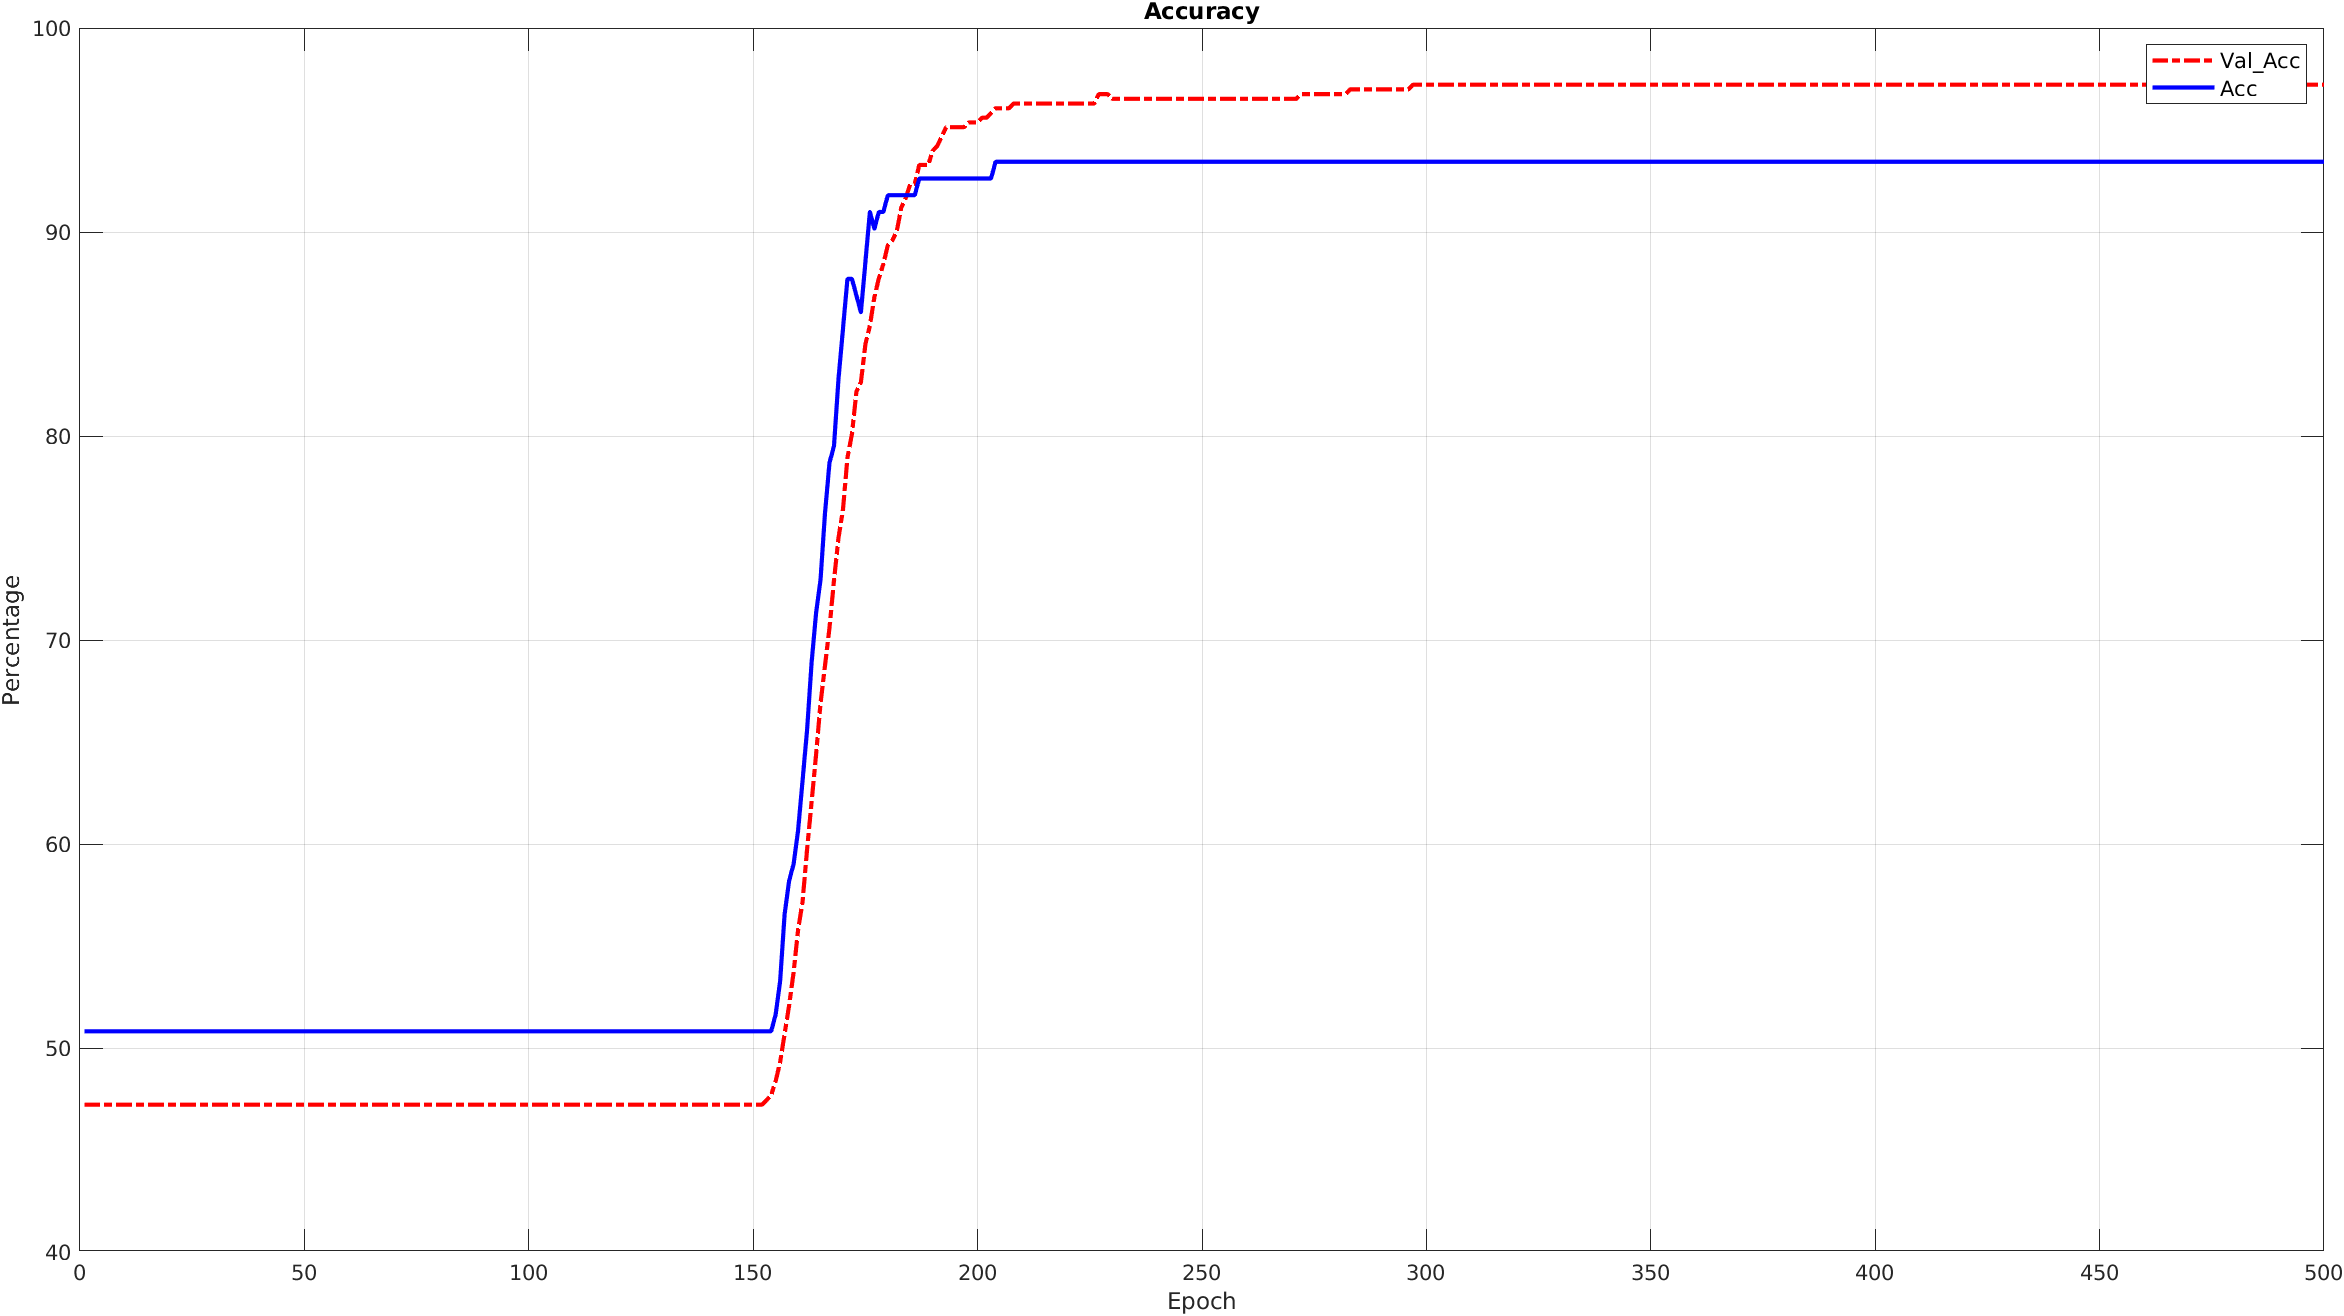
\includegraphics[width=\linewidth]{img/Monk3_accuracy_Reg.png}
        %\subcaption{Accuracy}
    \end{minipage}
    \caption{MSE and accuracy for MONK’s 3 regularized.}
\end{figure}



\subsection{Cup results}

\subsubsection{Validation schema}

At the beginning, we splitted the dataset in training set and test set with 80\% for training and 20\% for test. For the selection of the best model, we decided to use k-fold cross validation with k equals three. In the end we chose the best models among all the models trained during the grid search step. We used stochastic, mini-batch and batch gradient descent and we figured out that the batch type had smoother learning curves.

\subsubsection{Screening phase}

Firstly we tried networks with single hidden layer and we noticed that they had good results. For this reason we tuned the hyper-parameters for this type of network through grids search.
Then we chose MEE as the loss function for validation and test set, we trained the network with MSE but we plot the results with MEE to be comparable with the learning curves of test and validation set.
Next, we focused on find some variant of the network with more hidden layer, we did hyper-parameters tuning through grids search.

\subsubsection{Explored hyper-parameters}
At the beginning, we have done grids search with large interval and high step among them. When we found the right interval we started grids search for each combination of the values:

\begin{itemize}
	\item Unit $\in$ \{25, 200\} with step $\in$ \{25, 50\};
	\item Learning rate $\in$ \{0.0001, 0.01\} with step $\in$ \{0.0001, 0.001\};
	\item Lambda $\in$ \{0, 0.004\} with step $\in$ \{0.0001,  0.0005\};
	\item Momentum $\in$ \{0, 0.8\} with step $\in$ \{0.05,  0.1\}.
\end{itemize}
\vspace{0.3cm}
We used \texttt{tanh} activation function for all hidden layer and \texttt{linear} activation function in the output layer. \texttt{Tanh} was chosen because it had the best result among other results we obtained in previous grid search. \texttt{Linear} was chosen because is often used as output layer activation function for regression problem.

\subsubsection{Grid search result}
The table \ref{tab:best_nets} reports the average of the value found for TR, VS and TS during the k-fold cross validation with k equals three.   
\begin{center}
\small\addtolength{\tabcolsep}{-3pt}
\begin{table}[h!]
	\centering
	\begin{tabular}{|c|c|c|c|c|c|c|c|}
		\hline
		\textbf{Layer}& \textbf{Units}& \textbf{Learning rate} & \multicolumn{1}{l|}{\textbf{Lambda}} & \textbf{Momentum} & \textbf{Error TR}& \textbf{Error VS}& \textbf{Error TS}\\ \hline
			1 & 75 & 0.00450 & 0.00001 & 0.6  & 0.9676 & 1.1202 & 1.2151  \\
			1 & 100 & 0.00087 & 0.0000 & 0.8  & 0.9832 & 1.2750 &  1.2662\\
			1 & 100 & 0.00097 & 0.0000 & 0.8  & 0.9851 & 1.2759 &  1.2786\\
			1 & 100 & 0.00500 & 0.0000 & 0.5  & 0.9859 & 1.2845 & 1.2784 \\
			1 & 100 & 0.00500 & 0.0000 & 0.7  & 0.9752 & 1.2654 & 1.2569 \\
			1 & 100 & 0.00500 & 0.00001 & 0.6  & 0.8731& 1.2412 & 1.2375 \\
			2 & 150 & 0.00875 & 0.0002 & 0.8  & 0.8467 & 1.1332 &  1.1372 \\
			5 & 375 & 0.00450 & 0.0001 & 0.7  & 0.6323 & 1.1341 &  1.1341 \\
		  \hline
	\end{tabular}
		\caption{Best networks configuration with MEE.}
		\label{tab:best_nets}
\end{table}
\end{center}
The two models with more than one hidden layers have the following structure:
\begin{itemize}
	\item Two hidden layer: 100-50-2 (see fig. \ref{img::twolayer});
	\item Five hidden layer: 100-100-75-50-50-2 (see fig. \ref{img::fivelayer}).
\end{itemize}

\vspace{0.5cm}
\begin{figure}[H]
	\centering
	\begin{minipage}[t]{0.5\linewidth}
		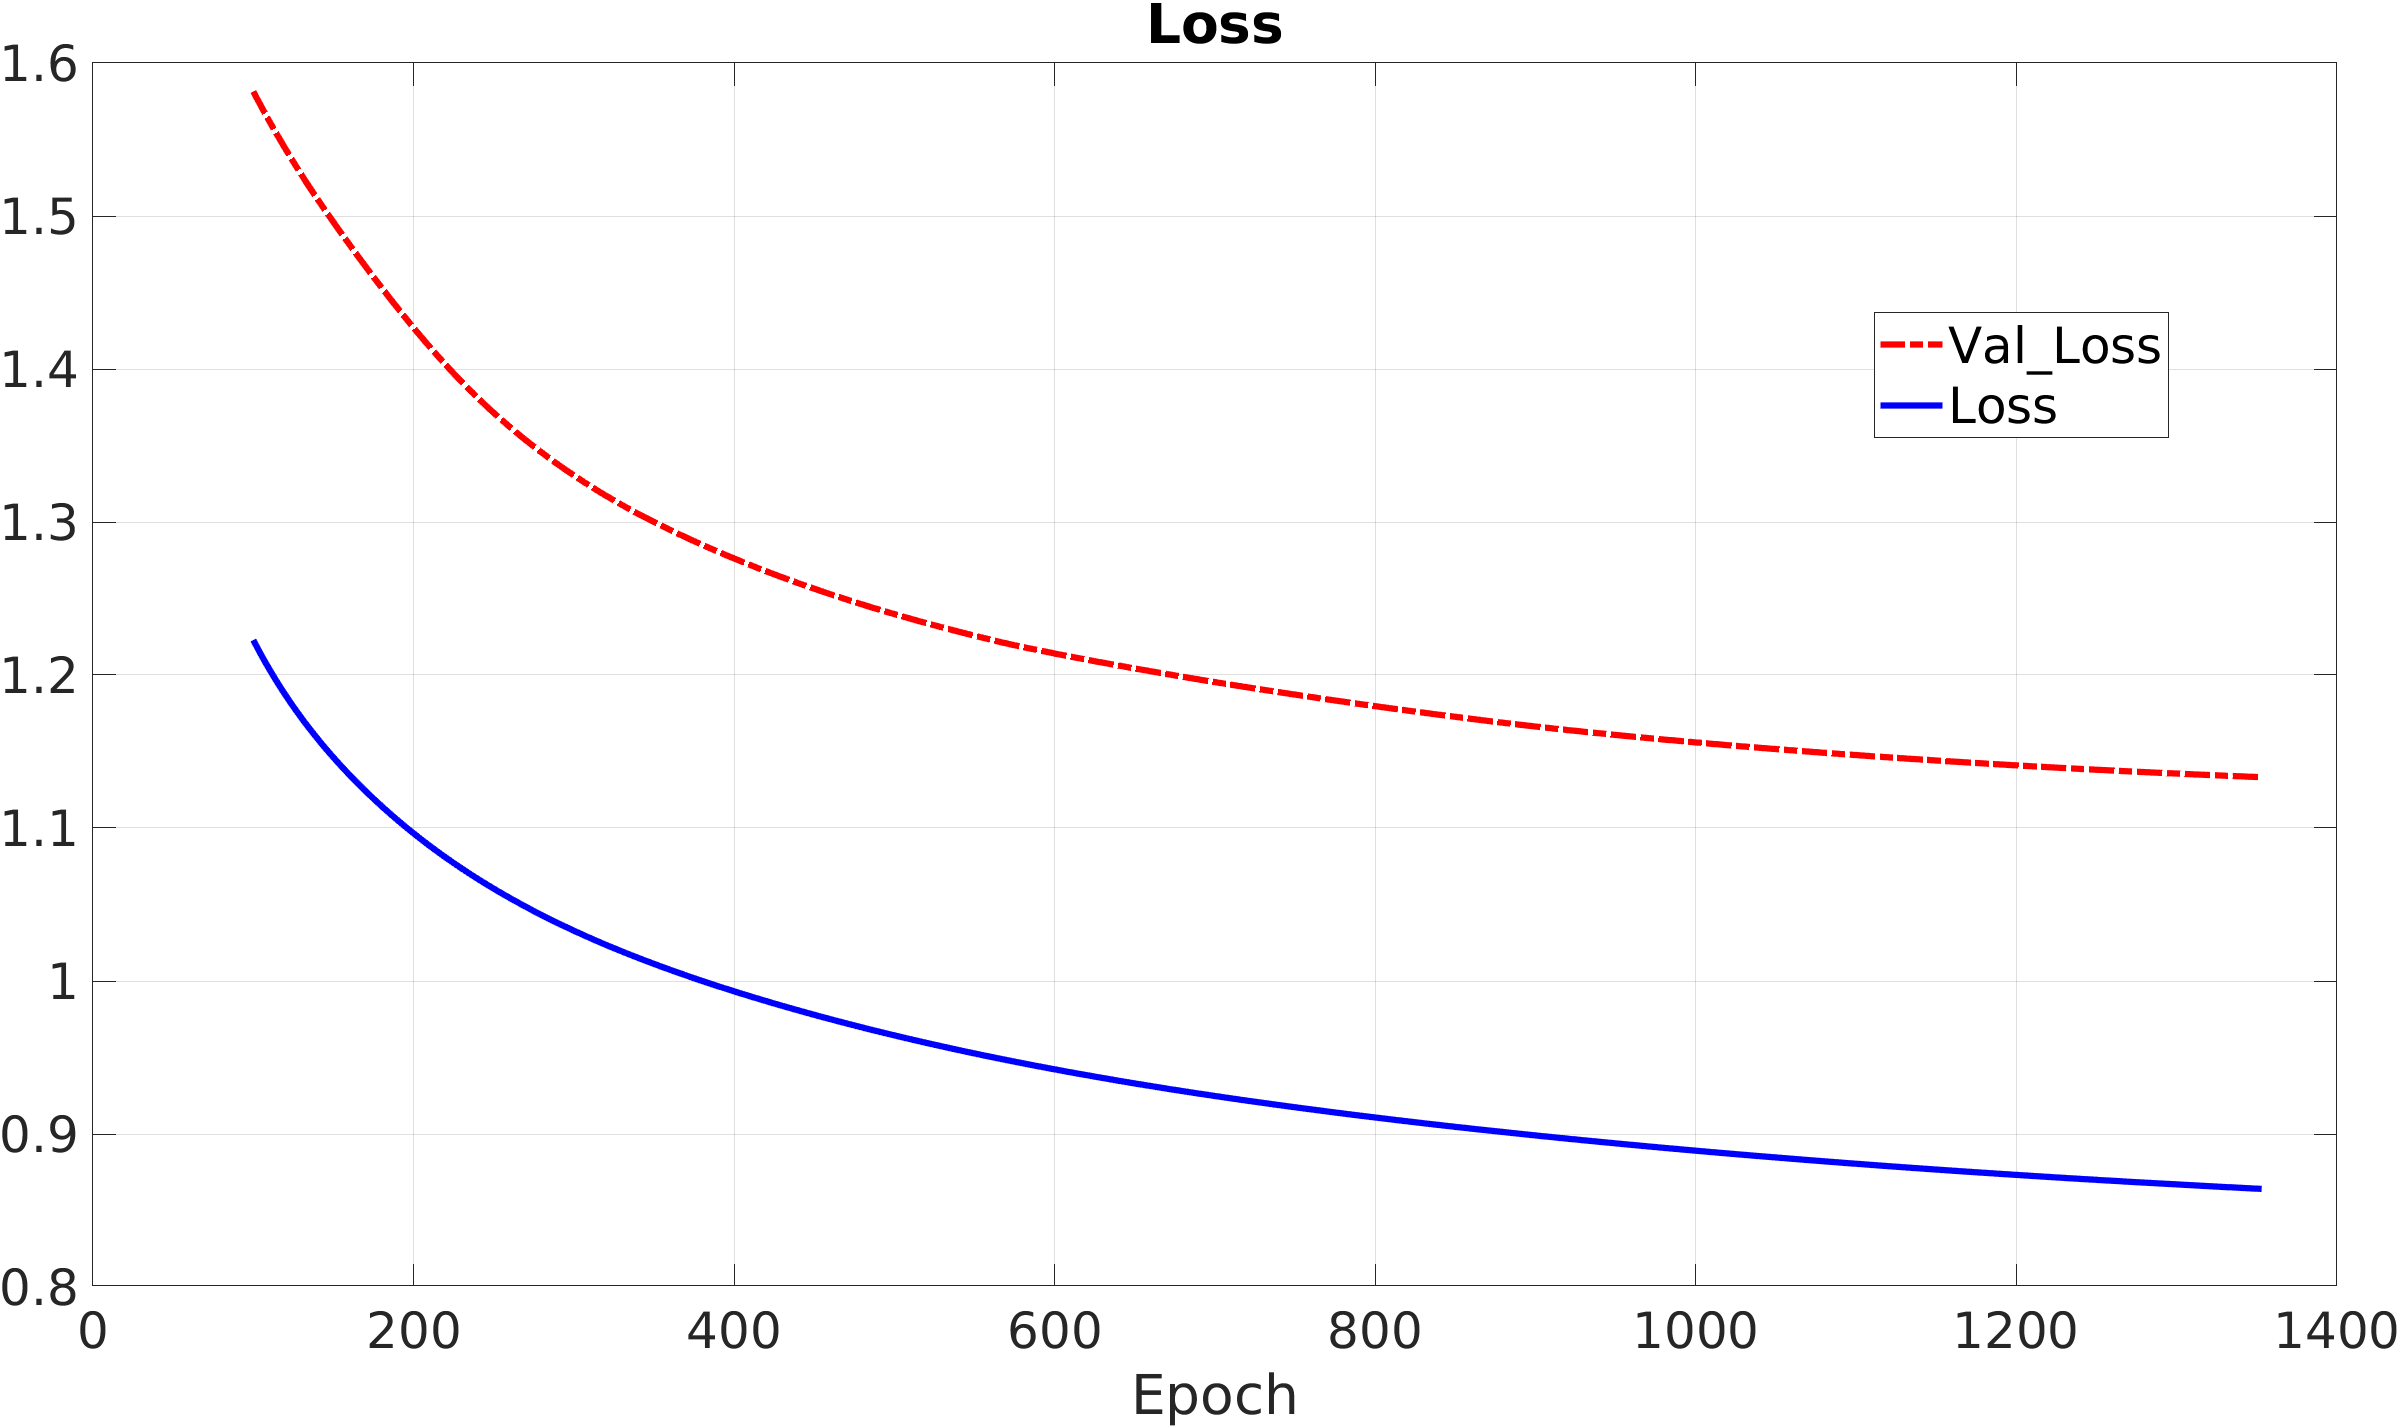
\includegraphics[width=\linewidth]{img/Cup_loss_Reg_Zoom_2l.png}
		\caption{MEE two hidden layer model}
		\label{img::twolayer}
	\end{minipage}%
	\begin{minipage}[t]{0.5\linewidth}
		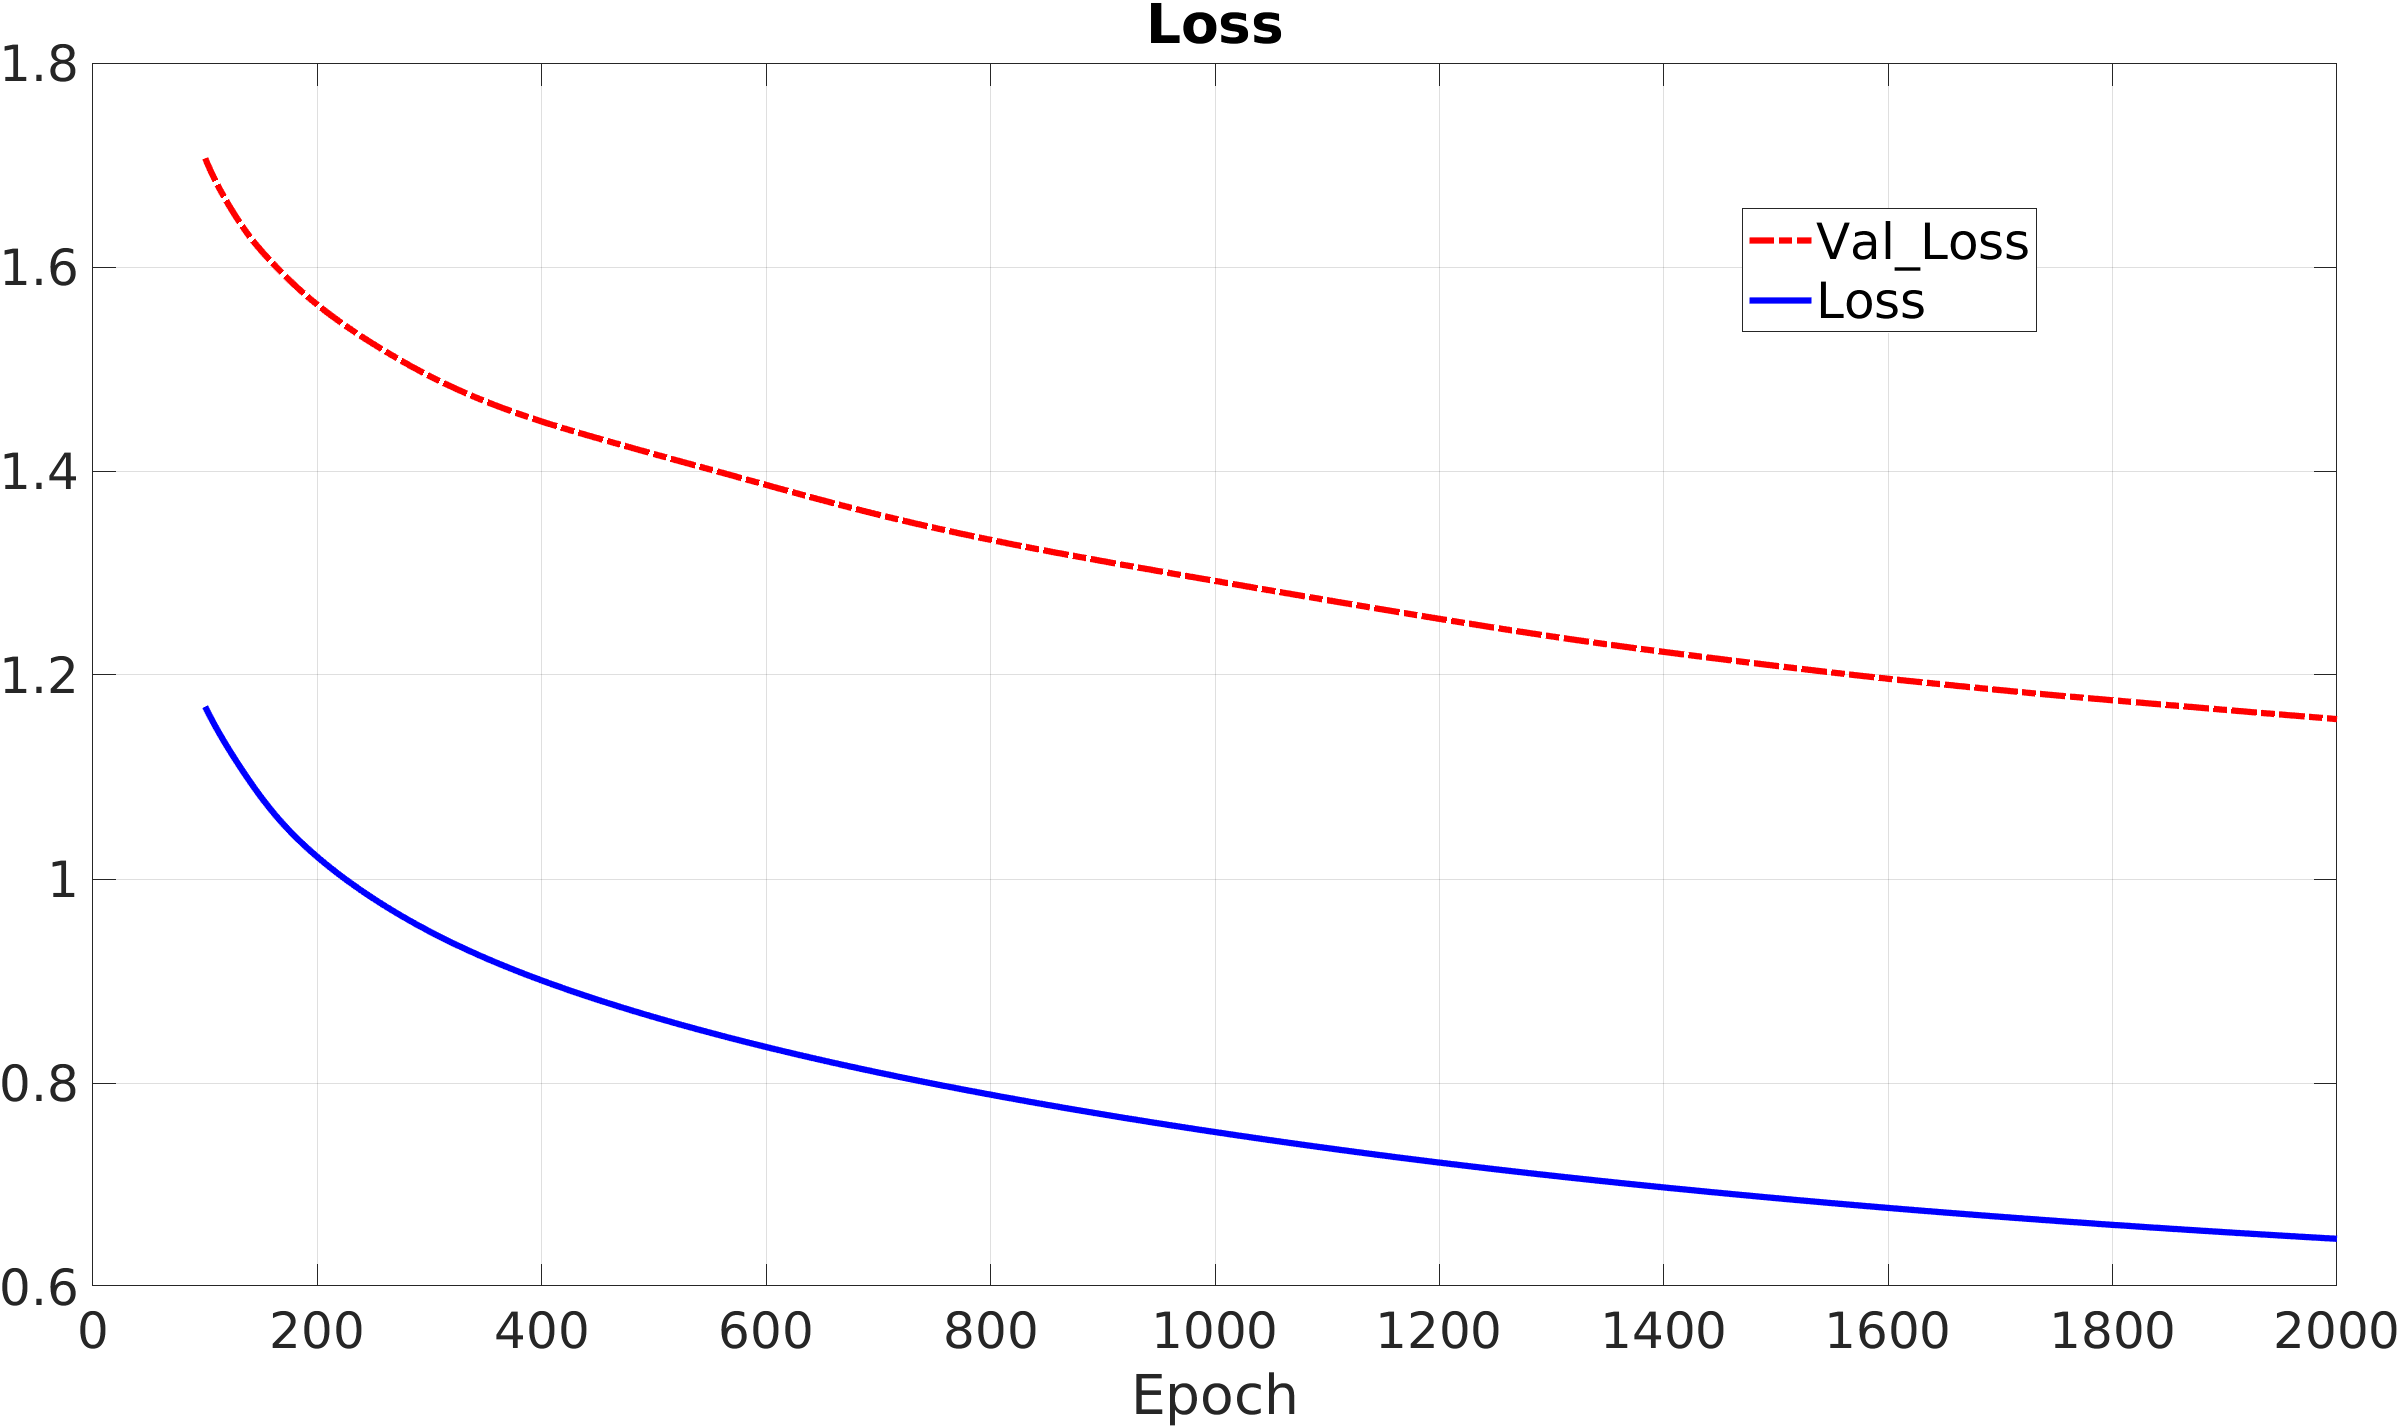
\includegraphics[width=\linewidth]{img/Cup_loss_Reg_Zoom_5l.png}
		\caption{MEE five hidden layer model}
		\label{img::fivelayer}
	\end{minipage}
\end{figure}

\subsubsection{Computing time}
We have developed a parallel grid search that allow us to take advantage of all core of our CPUs automatically. All the computation where launched on the following machine:
\begin{itemize}
	\item Intel i7-8500Y, 1.5GHz;
	\item Intel i7-4720HQ, 2.6GHz.
	
\end{itemize}

The project was developed in C++ and the computational time and memory had to be strictly controlled.
The time it takes to train on the MONK dataset with 800 epoch is 1.5 second, for the ML CUP dataset with 8000 epoch and 75 units is 1.10 minutes.

\subsubsection{Comparisons}
We have tried different neural networks with different number of layer and distinct type of gradient descent (stochastic, mini-batch and batch). We figured out that the number of layers does not significantly affect network generalization performance, moreover with batch gradient descent we got the best learning curve.

\subsubsection{Chosen model}
The final model was chosen from the best models found after the grid search (table \ref{tab:best_nets}), it has the following hyperparameters (table \ref{tab:best_net}) and MEE error for training set, validation set and test set.
We achieved an average MEE of 1.2093 on our test set, taken as an average of seven
different trainings of the networks (to avoid the bias due to the random weight
initialization).
\begin{center} 
\small\addtolength{\tabcolsep}{-3pt}
\begin{table}[h!]
	\centering
	\begin{tabular}{|c|c|c|c|c|c|c|c|}
		\hline
		\textbf{Layer}& \textbf{Units}& \textbf{Learning rate} & \multicolumn{1}{l|}{\textbf{Lambda}} & \textbf{Momentum} & \textbf{Error TR}& \textbf{Error VS}& \textbf{Error TS}\\ \hline
		1 & 75 & 0.00450 & 0.00001 & 0.6  & 0.9676 & 1.1202 & 1.2093  \\
		\hline
	\end{tabular}
	\caption{Best network configuration with MEE.}
	\label{tab:best_net}
\end{table}
\end{center}

We chose it because it was the model that performed better in the validation set. Also its learning curve was smooth and stable.
The learning curve, also with an enlargement, is shown in the figure \ref{img:best}.


\begin{figure}[H]
    \centering
    \begin{minipage}[t]{0.5\linewidth}
        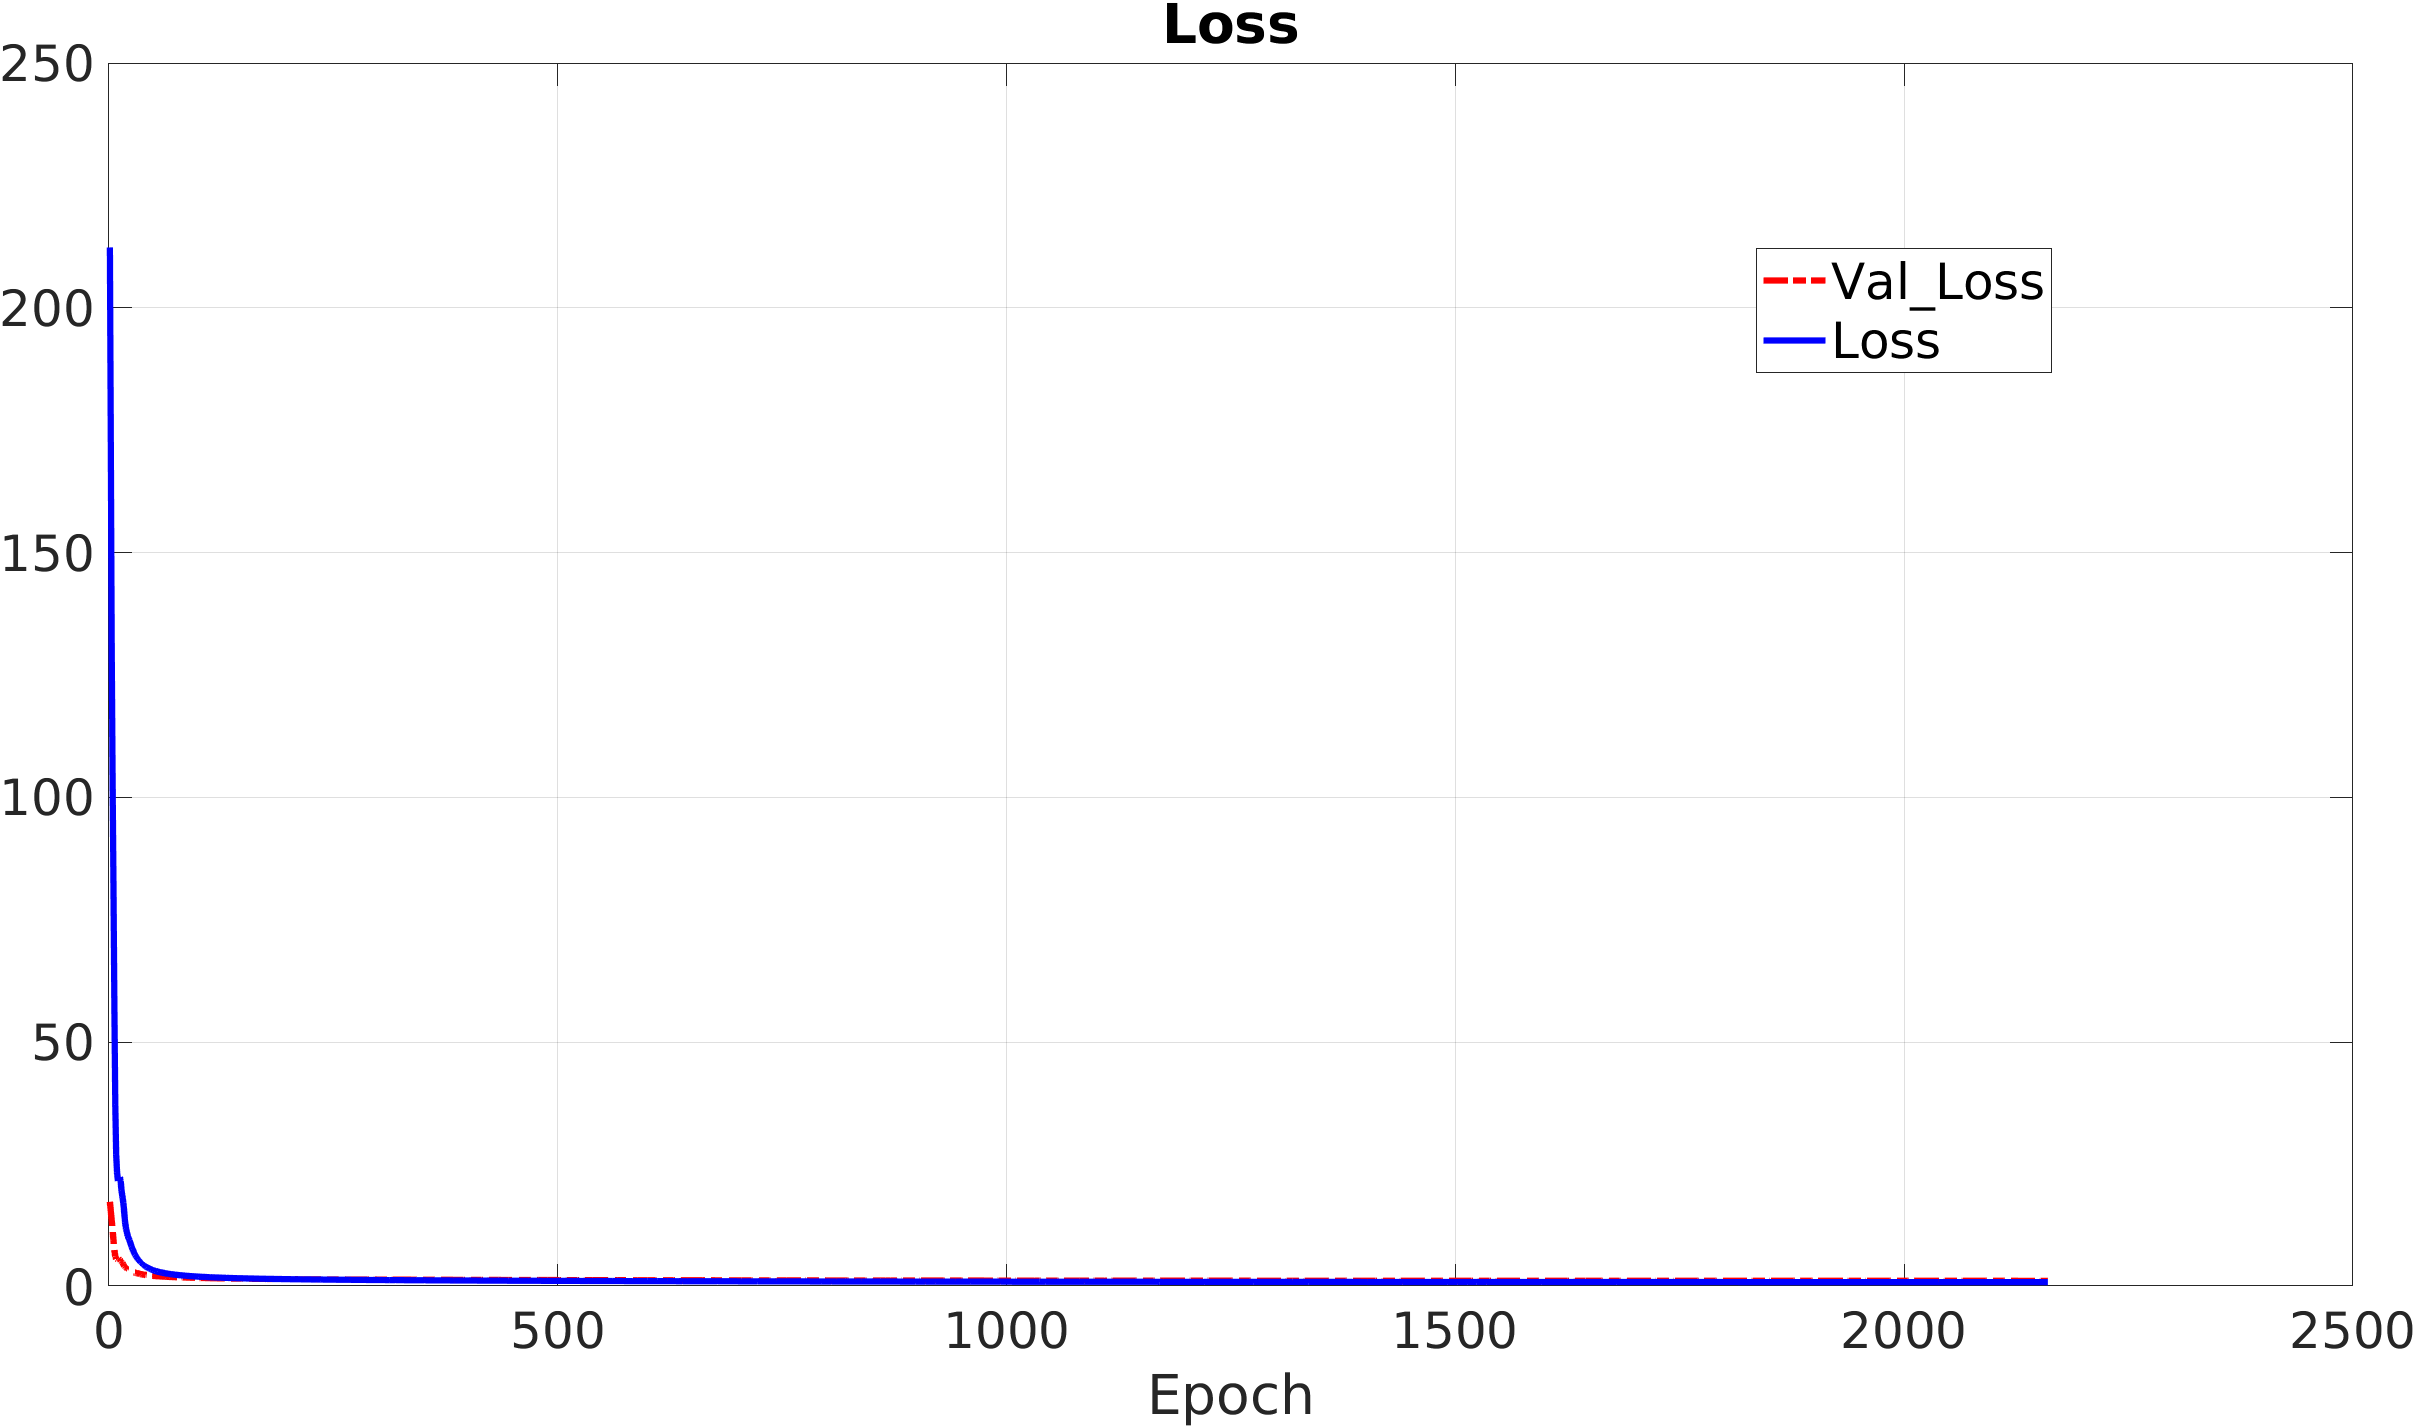
\includegraphics[width=\linewidth]{img/Cup_loss_Reg_noZoom.png}
        %\subcaption{MSE}
    \end{minipage}%
    \begin{minipage}[t]{0.5\linewidth}
        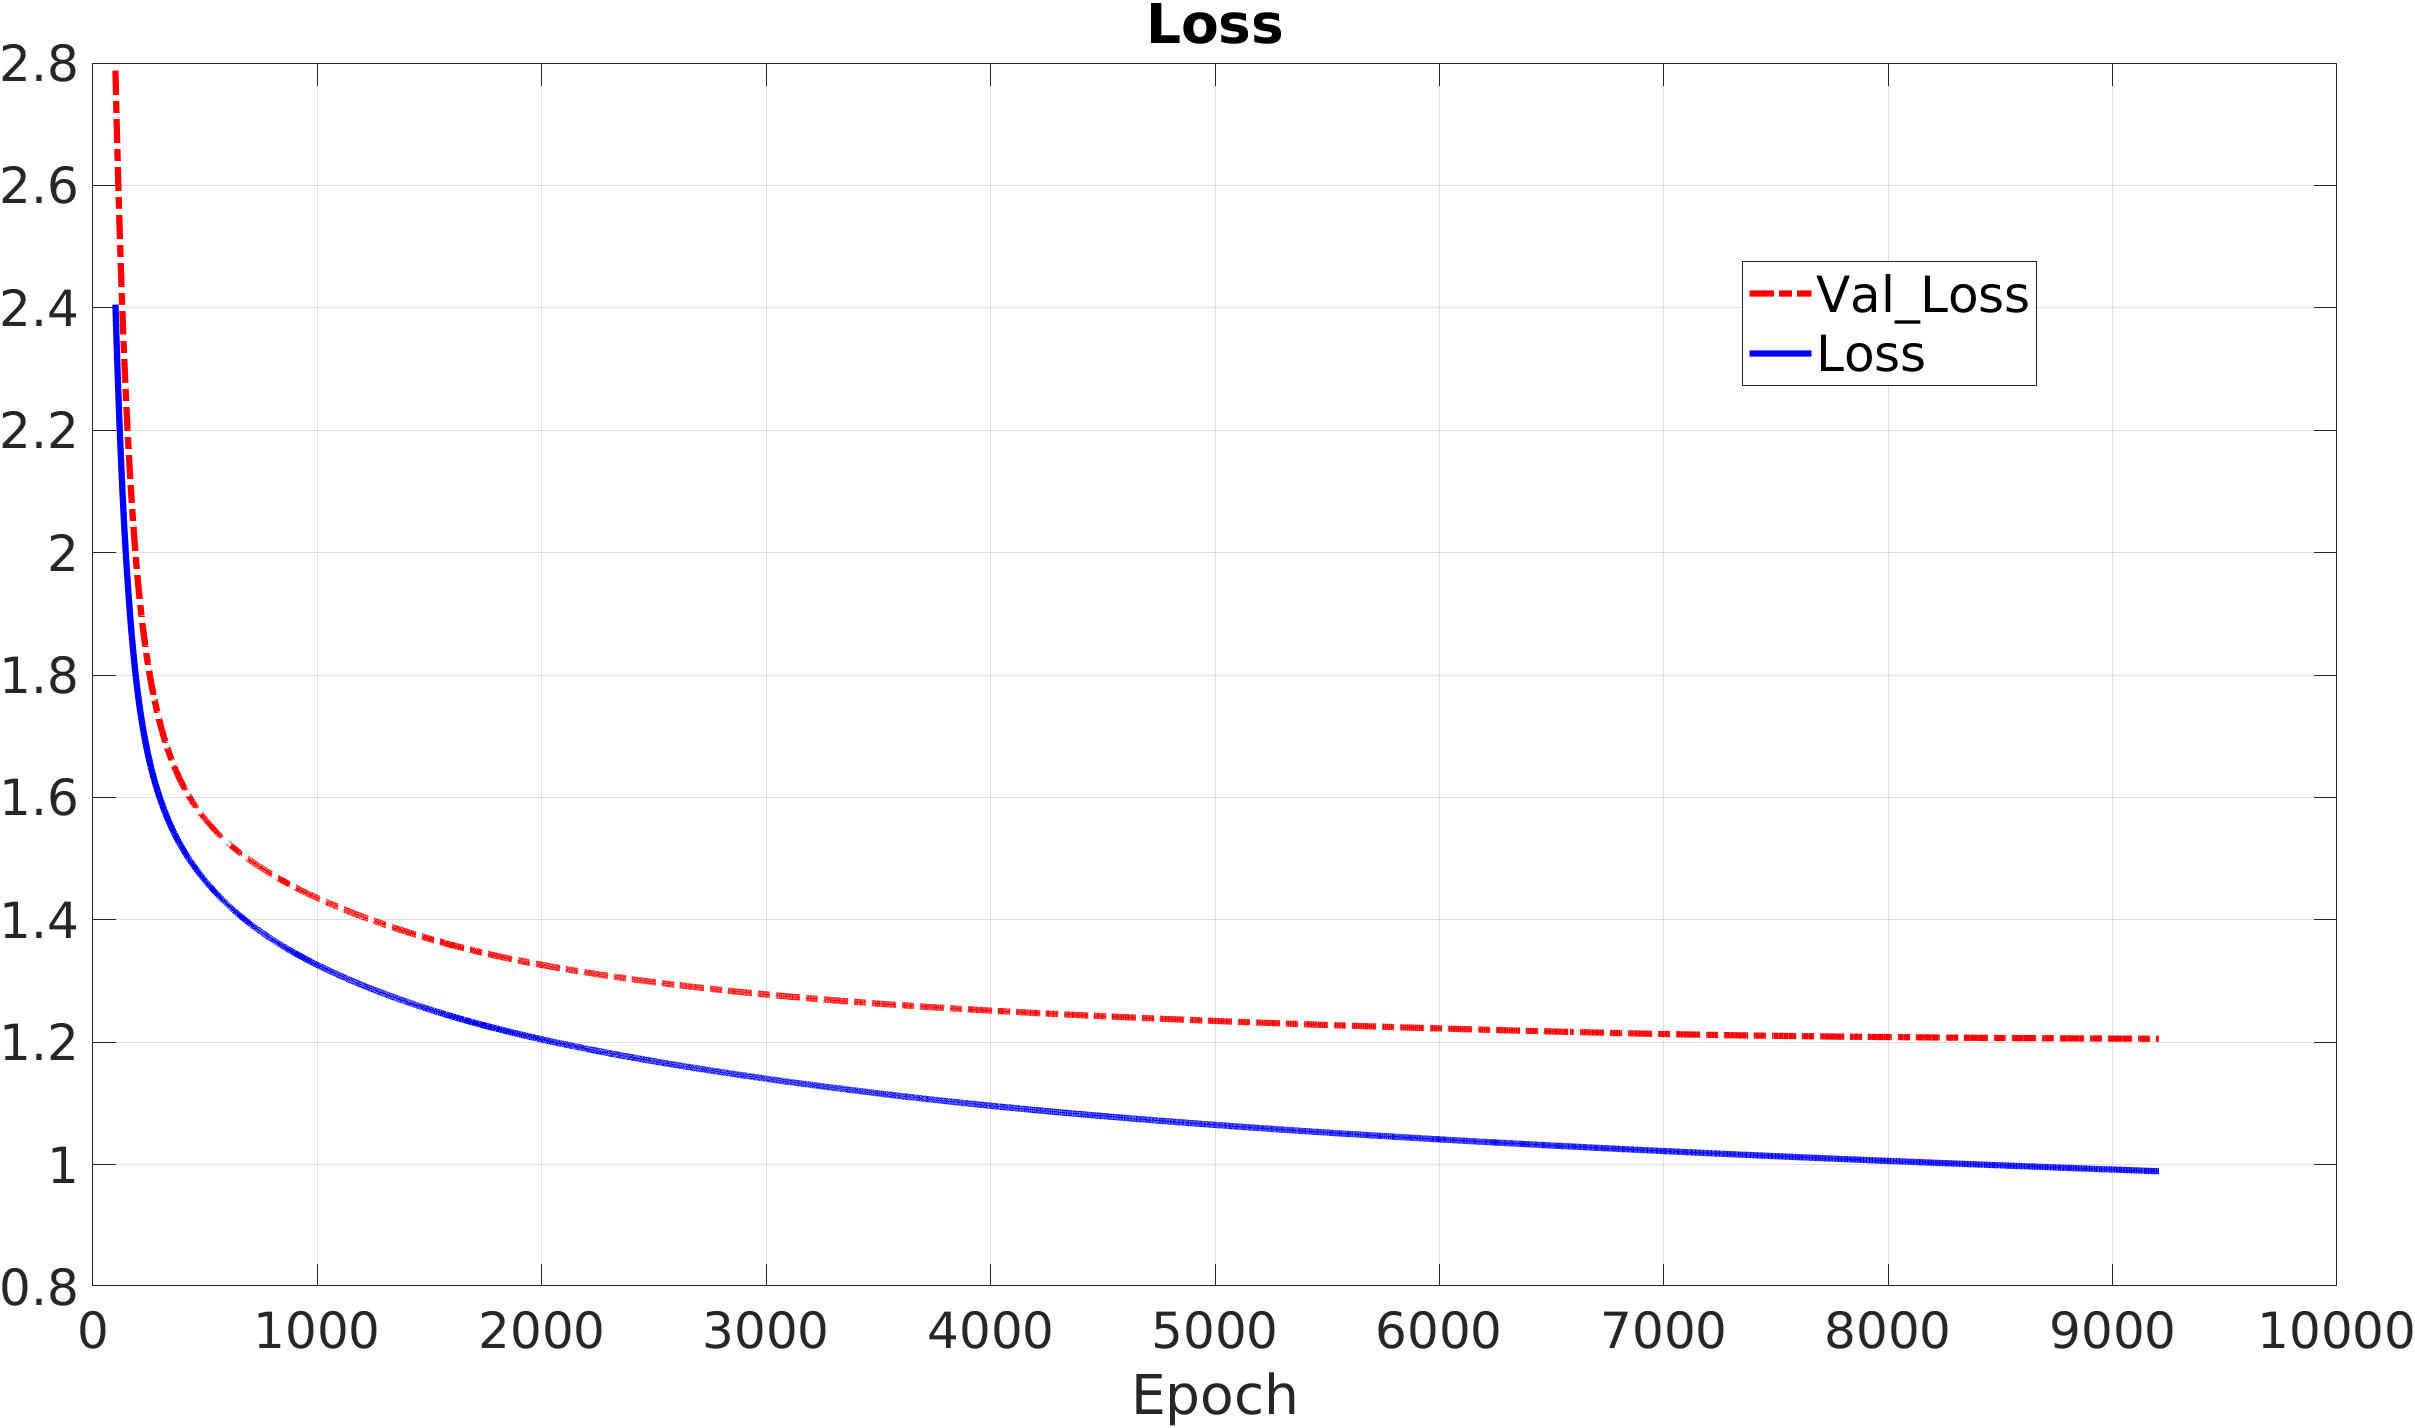
\includegraphics[width=\linewidth]{img/Cup_loss_Reg_Zoom.png}
        %\subcaption{Accuracy}
    \end{minipage}
    \caption{MEE and zoomed MEE for ML cup regularized.}
    \label{img:best}
\end{figure}




\section{Introduction}
Our goal is to create a Neural Network model simulator and apply it to MONK's classification problems and the ML CUP regression problem. 
We developed a library with the aim of build, training and test feedforward neural networks using back-propagation and multiple version of gradient descent: stochastic/online, mini-batch and batch with Nesterov Momentum and weight decay as regularization and using various activation functions and loss functions. 
Our assumption was to find the best model for each problem, this has been reached by looking for a smooth  and compact loss function. This aim has been pursued using grid search technique with k-fold cross validation. We paid attention not to commit overfitting using regularization technique such as weight decay. 
\section{Method}
\subsection{"Code"}
\subsection{"Code"}











Briefly (short part) describe what you developed and how:
• The code (for type A implementation) or the used simulator(s) (for type B). 
◦ The used tools/libraries (if any)
◦ Software overview and the software design choices (if interesting)
◦ Implementation choices: a  summary of the choices (e.g. architecture/s, training algorithm/s, type of activation function/s, batch/on-line/mb, regularization schema, stop condition)
◦ The novelties (if any) but not the standard approaches (do not describe the algorithms/models we already described in the lectures). Use references for the source of information. 
• Preprocessing procedure (if any) [details may be postponed to Section 3]
• Validation schema (model selection and evaluation schema) for the Experimental part: report data splitting  TR/VL/TS (% data for each set and/or the K values of the k-fold CV) [details may be postponed to Section 3]
• Type of preliminary trials pursued (often summarized by text) [details may be postponed to Section 3]



Each figure/table should be referenced as in the following, see Fig. 1. 
Do not use figure/table without a number. Do not write “see the next figure” (which one?).
Tables and plots have always a caption. All of the Figures and Tables should be cited in order, including those in the Appendix. (which should be cited as, for example, Fig. A.1, and Table A.1).

\end{document}